\documentclass{article}

\usepackage{graphics}
\usepackage{graphicx}
\usepackage{amsmath,amssymb,amsthm}
%\usepackage{subeqnarray}
%\usepackage{easybmat}
\usepackage{subfigure}



%\usepackage{HA-prosper}
%\usepackage[dvips,letterpaper]{geometry}

\newtheorem{property}{Property}[section]
\newtheorem{theorem}{Theorem}[section]
\newtheorem{definition}[theorem]{Definition}
\newtheorem{proposition}[theorem]{Proposition}
\newtheorem{lemma}[theorem]{Lemma}
\newtheorem{corollary}[theorem]{Corollary}



\def\R{\mathbb{R}}
\def\Rzero{\mathcal{R}_0}
\def\diag{\textrm{diag}}
\def\tr{\textrm{tr}}
\def\det{\textrm{det}}
\def\sgn{\textrm{sgn}}
\def\imply{$\Rightarrow$}

\title{Lecture Notes: MATH 3530}
\date{\today}
\begin{document}
\maketitle
\tableofcontents
%\newpage

\part{Introduction}

{\bf Mathematical modeling:} an idealization of the real-world problems and never a completely accurate representation
\begin{itemize}
\item Identify the most important processes governing the problem (Theoretical assumptions)
\item Identify the state variables (quantities studied)
\item Identify the basic principles that govern the state variables (Physical
Laws, interactions, $\dots$)
\item Express mathematically these principles in terms of state variables (Choice of the formalism)
%\item Units for each state variable
\item Identify and evaluate the values of parameters
\item Make sure of the consistence of units
\end{itemize}

{\bf Different types of biological problems:} mathematical biology encompass several domains such that 
\begin{itemize}
\item Ecology (Predator-Prey system, Populations in competition $\dots$)
\item Etology 
\item Epidemiology (Propagation of infectious diseases)
\item Physiology (Neuron, cardiac cells, muscular cells)
\item Immunology
\item Cell biology
\item Structural biology
\item Molecular biology
\item Genetics (Spread of genes in a population)
\item $\dots$
\end{itemize}


{\bf Different approaches exist to represent a problem:}
How to represent a problem?
\begin{itemize}
\item Static vs dynamic
\item Stochastic vs Deterministic
\item Continous vs Discrete
\item Homogeneous vs Detailed
\end{itemize}
{\bf Different formalisms}
ODE, PDE, DDE, SDE, Integral equation, integro-differential equations, Markov Chains, Game theory, Graph theory, Cellular automata, L-systems $\dots$
\begin{center}
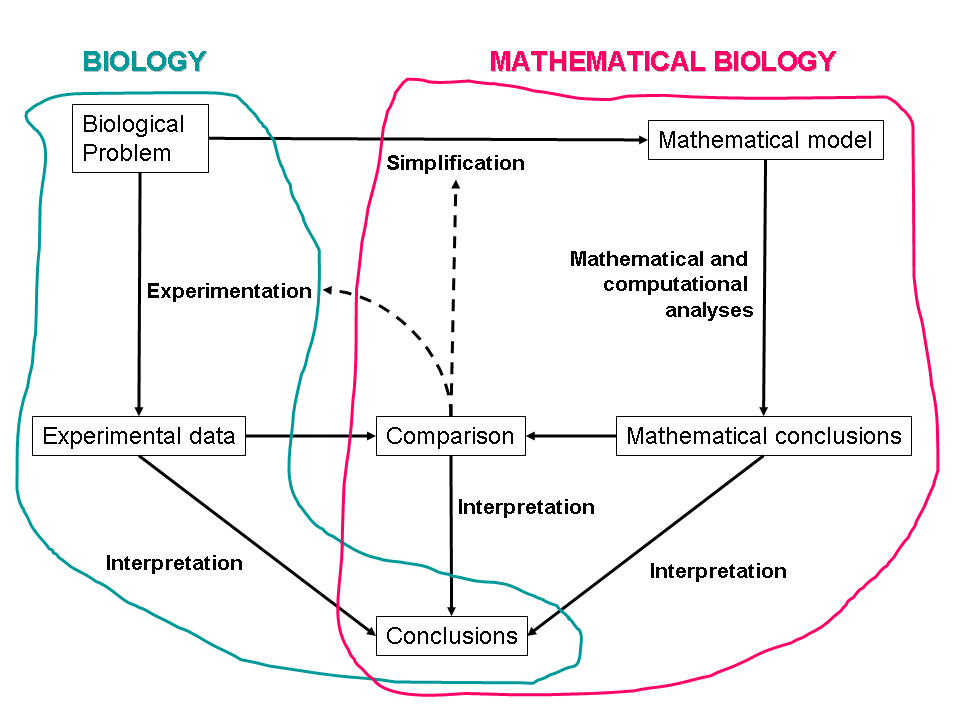
\includegraphics[width=.8\textwidth]{figs_steph/FigureMathBio}
\end{center}


\part{Difference equations}
Some characteristics of difference equations
\begin{itemize}
\item changes of states are descibed over discrete intervals. Length of the discrete interval is some fixed length $\Delta t$: states of a system are modeled at the discrete time $t=0,\Delta t, 2\Delta t, \dots$
\item recurrence relation
\item evolutionary character or not
\item to describe populations whose generations do not overlap:
\end{itemize}


\section{General definitions}
Notation: time interval is often simplified $\Delta t=1$, and the state of the system at time $t$ as $x_t$.


\begin{definition}
A difference equation of order $k$ has the form $$f(x_{t+k},x_{t+k-1},\dots,x_{t+1},x_t,t)=0\quad t=0,1,\dots,$$
where $f$ is a real-valued function of the real variable $x_t$ through $x_{t+k}$ and $t$.
\end{definition}
\begin{definition}
The order of a difference equation is the difference between the largest and the smallest arguments $k$ appearing in it.
\end{definition}
The order $k$ of the equation is the number of previous generations that directly influence the value of $x$ in a given generation.



\begin{definition}
The difference equation is called autonomous if $f$ does not depend explicitly on $t$ and it is called nonautonomous otherwise.
\end{definition}

Let 
$$x_{t+k}+a_1 x_{t+k-1}+a_2 x_{t+k-2}+\dots +a_{k-1} x_{t+1}=b_t \quad t=0,1,\dots$$

\begin{definition}
If the coefficients $a_j$, $j=1,\dots , k$ are constant or depend on $t$ but {\bf do not depend on the state variables}, then the difference equation is said to be {linear}; otherwise, it is to be nonlinear. 
\end{definition}

\begin{definition}
If the difference equation is linear and $b_t=0$ for all $t$, then it is said to be homogeneous; otherwise, it is said to be nonhomogeneous.
\end{definition}



\begin{definition}
A solution of the difference equation
$$f(x_{t+k},x_{t+k-1},\dots,x_{t+1},x_t,t)=0\quad t=0,1,\dots,$$
is a function $x_t$, $t=0,1,2,\dots$ such that when substituted into the equation makes it a true statement.
\end{definition}



\section{First-order linear difference equation}
\begin{proposition}
Let a first-order linear homogeneous difference equation with constant coefficients
$$x_{t+1}=ax_t$$
If $x_0$ (initial value) is known, the solution is unique and is
$$x_t=a^tx_0$$
\end{proposition}

\begin{quote}
Proof:
$$x_1=ax_0$$
$$x_2=ax_1=aax_0=a^2 x_0$$
$$x_3=ax_2=aaax_0=a^3x_0 \dots$$

In general, $x_t=a^tx_0$
\end{quote}


{\bf Asymptotic behavior} of the solution depends on the value of $a$:
\begin{itemize}
\item $0<a<1$ then $\lim_{t\rightarrow \infty}x_t=0$
\item $a=1$ then $x_t=x_0$ $\forall t$
\item $a>1$ then $\lim_{t\rightarrow \infty}x_t=+\infty$
\end{itemize}


In general
\begin{itemize}
\item $|a|<1$ $x_t$ converges to 0.
\item $a=1$ $x_t$ is constant.
\item $|a|>1$ $x_t$ diverges (either approaches infinity or oscillates).
\end{itemize}


\begin{proposition}
Let a first-order linear homogeneous difference equation
$$x_{t+1}=a(t)x_t \quad t=0,1,2,\dots$$
If $x_0$ (initial value) is known, the solution is unique and is
$$x_t=\left [\prod_{i=0}^{t-1} a(i)\right ]x_0$$
\end{proposition}

\begin{quote}
Proof: Let prove by mathematical induction that $P(t)$ hold $\forall t\in \mathbb{Z}^+$ 
$$P(t): \quad x_t=\left [\prod_{i=0}^{t-1} a(i)\right ]x_0$$
\begin{itemize}
\item Verify that $P(1)$ is true
$$x_1=a(0)x_0$$
\item Assume that $P(\cdot)$ is true at rank $t$: $x_t=\left [\prod_{i=0}^{t-1} a(i)\right ]x_0$. Now express $P(t+1)$
$$x_{t+1}=a(t)x_t=\underbrace{a(t)\left [\prod_{i=0}^{t-1} a(i)\right ]}_{\prod_{i=0}^{t} a(i)}x_0,$$
then $P(t+1)$ is true.
\end{itemize}
By the principle of mathematical induction, we conclude that $$ x_t=\left [\prod_{i=0}^{t-1} a(i)\right ]x_0, \forall t\in \mathbb{Z}^+$$

\end{quote}


\begin{proposition}\label{Prop:FirstLinNonH}
Let a first-order linear nonhomogeneous difference equation
$$x_{t+1}=a(t)x_t + b(t)\quad t=0,1,2,\dots$$
If $x_0$ (initial value) is known, the solution is unique and is
$$x_t=\left [\prod_{i=0}^{t-1} a(i)\right ]x_0 +b(t-1)+\sum_{i=0}^{t-2}\left [ \prod_{r=i+1}^{t-1} a(r) \right]b(i)$$
{\bf Special cases:}
\begin{itemize}
\item $x_{t+1}=a x_t + b(t)\quad x(0)=x_0$, then $$x_t=a ^t x_0 +\sum_{i=0}^{t-1} a^{t-i-1}b(i)$$
\item $x_{t+1}=a x_t + b \quad x(0)=x_0$, then 
$$x_t=\left \{ \begin{array}{ll}a ^t x_0 +b\left[\frac{a^t-1}{a-1}\right] & a\not =1\\  x_0 +bt & a =1
\end{array}
\right.$$
\end{itemize}
\end{proposition}


\begin{quote}
Proof: Let prove by mathematical induction that $x_t=\left [\prod_{i=0}^{t-1} a(i)\right ]x_0 +b(t-1)+\sum_{i=0}^{t-2}\left [ \prod_{r=i+1}^{t-1} a(r) \right]b(i)$ for all $t\in \mathbb{Z}^+$
\begin{itemize}
\item Verify at rank $t=2$: $x_1=a(0)x_0+b(0)$, then
$$x_2=a(1)x_1+b(1)=a(1)a(0)x_0+a(1)b(0)+b(1).$$
%Similarly for $x_3$
%$$x_3=a(2)x_2+b(2)=a(2)a(1)a(0)x_0+a(2)a(1)b(0)+a(2)b(1)+b(2)$$
\item Assume that $$x_t=\left [\prod_{i=0}^{t-1} a(i)\right ]x_0 +b(t-1)+\sum_{i=0}^{t-2}\left [ \prod_{r=i+1}^{t-1} a(r) \right]b(i)$$
and express now $x_{t+1}$
$$x_{t+1}=a(t)x_t+b(t)=a(t)\left [ \left [\prod_{i=0}^{t-1} a(i)\right ]x_0 +b(t-1)+\sum_{i=0}^{t-2}\left [ \prod_{r=i+1}^{t-1} a(r) \right]b(i) \right ]+b(t)$$
$$x_{t+1}=\left [a(t)\prod_{i=0}^{t-1} a(i)\right ]x_0+a(t)b(t-1)+\sum_{i=0}^{t-2}\left [ a(t)\prod_{r=i+1}^{t-1} a(r) \right]b(i)+b(t)$$
$$x_{t+1}=\left [\prod_{i=0}^{t} a(i)\right ]x_0+\underbrace{a(t)b(t-1)+\sum_{i=0}^{t-2}\left [ \prod_{r=i+1}^{t} a(r) \right]b(i)}_{\sum_{i=0}^{t-1}\left [ \prod_{r=i+1}^{t} a(r) \right]b(i)}+b(t)$$
$x_{t+1}$ satisfies the relation.
\end{itemize}
By the principle of mathematical induction, we conclude that $$x_t=\left [\prod_{i=0}^{t-1} a(i)\right ]x_0 +b(t-1)+\sum_{i=0}^{t-2}\left [ \prod_{r=i+1}^{t-1} a(r) \right]b(i) \quad \forall t\in \mathbb{Z}^+$$
\end{quote}

\section{Second-order and higher-order linear equations}
\begin{definition}
The functions $x_t^1$, $x_t^2$,$\dots, x_t^k$ are said to be linearly independent for $t\geq t_0$ whenever 
$$a_1x^1_t+a_2x^2_t+\dots + a_kx^k_t=0$$
for all $t\geq t_0$, then we must have $a_1=a_2= \dots =a_k=0$.
\end{definition}

\begin{definition}
The Casoratian of $k$ functions $x_t^1$, $x_t^2$,$\dots, x_t^k$ is
$$C(x_t^1, x_t^2,\dots, x_t^k)=\det \left (
\begin{array}{cccc}
x_t^1 & x_t^2 & \dots & x_t^k\\
x_{t+1}^1 & x_{t+1}^2 & \dots & x_{t+1}^k\\
x_{t+2}^1 & x_{t+2}^2 & \dots & x_{t+2}^k\\
\vdots & & &\\
x_{t+k-1}^1 & x_{t+k-1}^2 & \dots & x_{t+k-1}^k\\
\end{array}\right )$$
\end{definition}

\begin{proposition}
If the Casoratian of $x_t^1$, $x_t^2$,$\dots, x_t^k$ satifies
$$C(x_t^1, x_t^2,\dots, x_t^k)\not =0 \quad \forall t$$
then $x_t^1$, $x_t^2$,$\dots, x_t^k$  are $k$ linearly independent functions.
\end{proposition}

\begin{definition}
A set of $k$ linearly independent solutions of a $k^{th}$ linear homogeneous difference equation is called a fundamental set of solutions.
\end{definition}

\begin{proposition}(Principle of superposition)
If $x_t^1$, $x_t^2$,$\dots, x_t^k$ are solutions a $k^{th}$ linear homogeneous difference equation then $$c_1x_t^1+c_2x_t^2+\dots, c_kx_t^k$$
is also solution of the $k^{th}$ linear homogeneous difference equation.
\end{proposition}

\begin{definition}
Let $\{x_t^1, x_t^2,\dots, x_t^k\}$ be a fundamental set of solutions of $k^{th}$ linear homogeneous difference equation. Then the general solution of the  $k^{th}$ linear homogeneous difference equation is given by $$x_t=\sum_{i=1}^kc_ix^i_t,$$ for arbitrary constants $c_i$, $i=1,\dots, k$
\end{definition}

\subsection{Second-order and higher-order linear homogeneous equations with constant coefficients}
The case of a second-order equation is derived to illustrate this subsection.

A second-order linear homogeneous equation with constant coefficients:
\begin{equation}\label{eq:SecLinHom}
a_0x_{t+2}+a_1x_{t+1}+ a_2 x_{t}=0
\end{equation}
To find two linearly independent solutions, $x_t^1$ and $x_t^2$: assume that solutions take the form of 
$x_t=\lambda ^t$ with $\lambda \not= 0$. Then substitute solution in \eqref{eq:SecLinHom}
$$a_0\lambda ^{t+2}+a_1\lambda ^{t+1}+ a_2 \lambda ^{t}=0,$$
$$a_0\lambda ^{2}+a_1\lambda + a_2 =0.$$

The equation $a_0\lambda ^{2}+a_1\lambda + a_2 =0$ is called the characteristic equation of \eqref{eq:SecLinHom}. The 2 roots of the characteristic equation, $\lambda_1$ and $\lambda_2$, are called the eigenvalues.

The general solution is a linear combination of the 2 solutions $x_t^1=\lambda_1^t$ and $x_t^2=\lambda_2^t$. The form of the general solution depends on the eigenvalues and there exist 3 cases:
\begin{itemize}
\item {\bf Eigenvalues are real and distinct:} $\lambda _1 \not = \lambda _2 $. The general solution is
$$x_t=c_1\lambda _1 ^t+c_2\lambda _2 ^t,$$
with $c_1$ and $c_2$ arbitrary constants.
\item {\bf Eigenvalues are real and equal:} $\lambda _1  = \lambda _2 $. Then the $2$ linearly independent solutions are  $x_t^1=\lambda _1^t$ $x_t^2=t\lambda _2^t$. 
The general solution is
$$x_t=c_1\lambda _1 ^t+c_2t\lambda _2 ^t,$$
with $c_1$ and $c_2$ arbitrary constants.
\item {\bf Eigenvalues are complex conjugates:} $\lambda _{1,2}=A\pm iB=r(\cos \phi \pm i \sin \phi)$, where $r=\sqrt{A^2+B^2}$ and $\phi=\arctan(B/A)$. The two lienarly independent solutions are $x^1=r^t\cos(t\phi)$ and $x^2=r^t\sin (t\phi)$.

Then the general solution is
$$x_t=c_1 r^t\cos(t\phi)+c_2r^t\sin (t\phi),$$
with $c_1$ and $c_2$ arbitrary constants.
\begin{center}
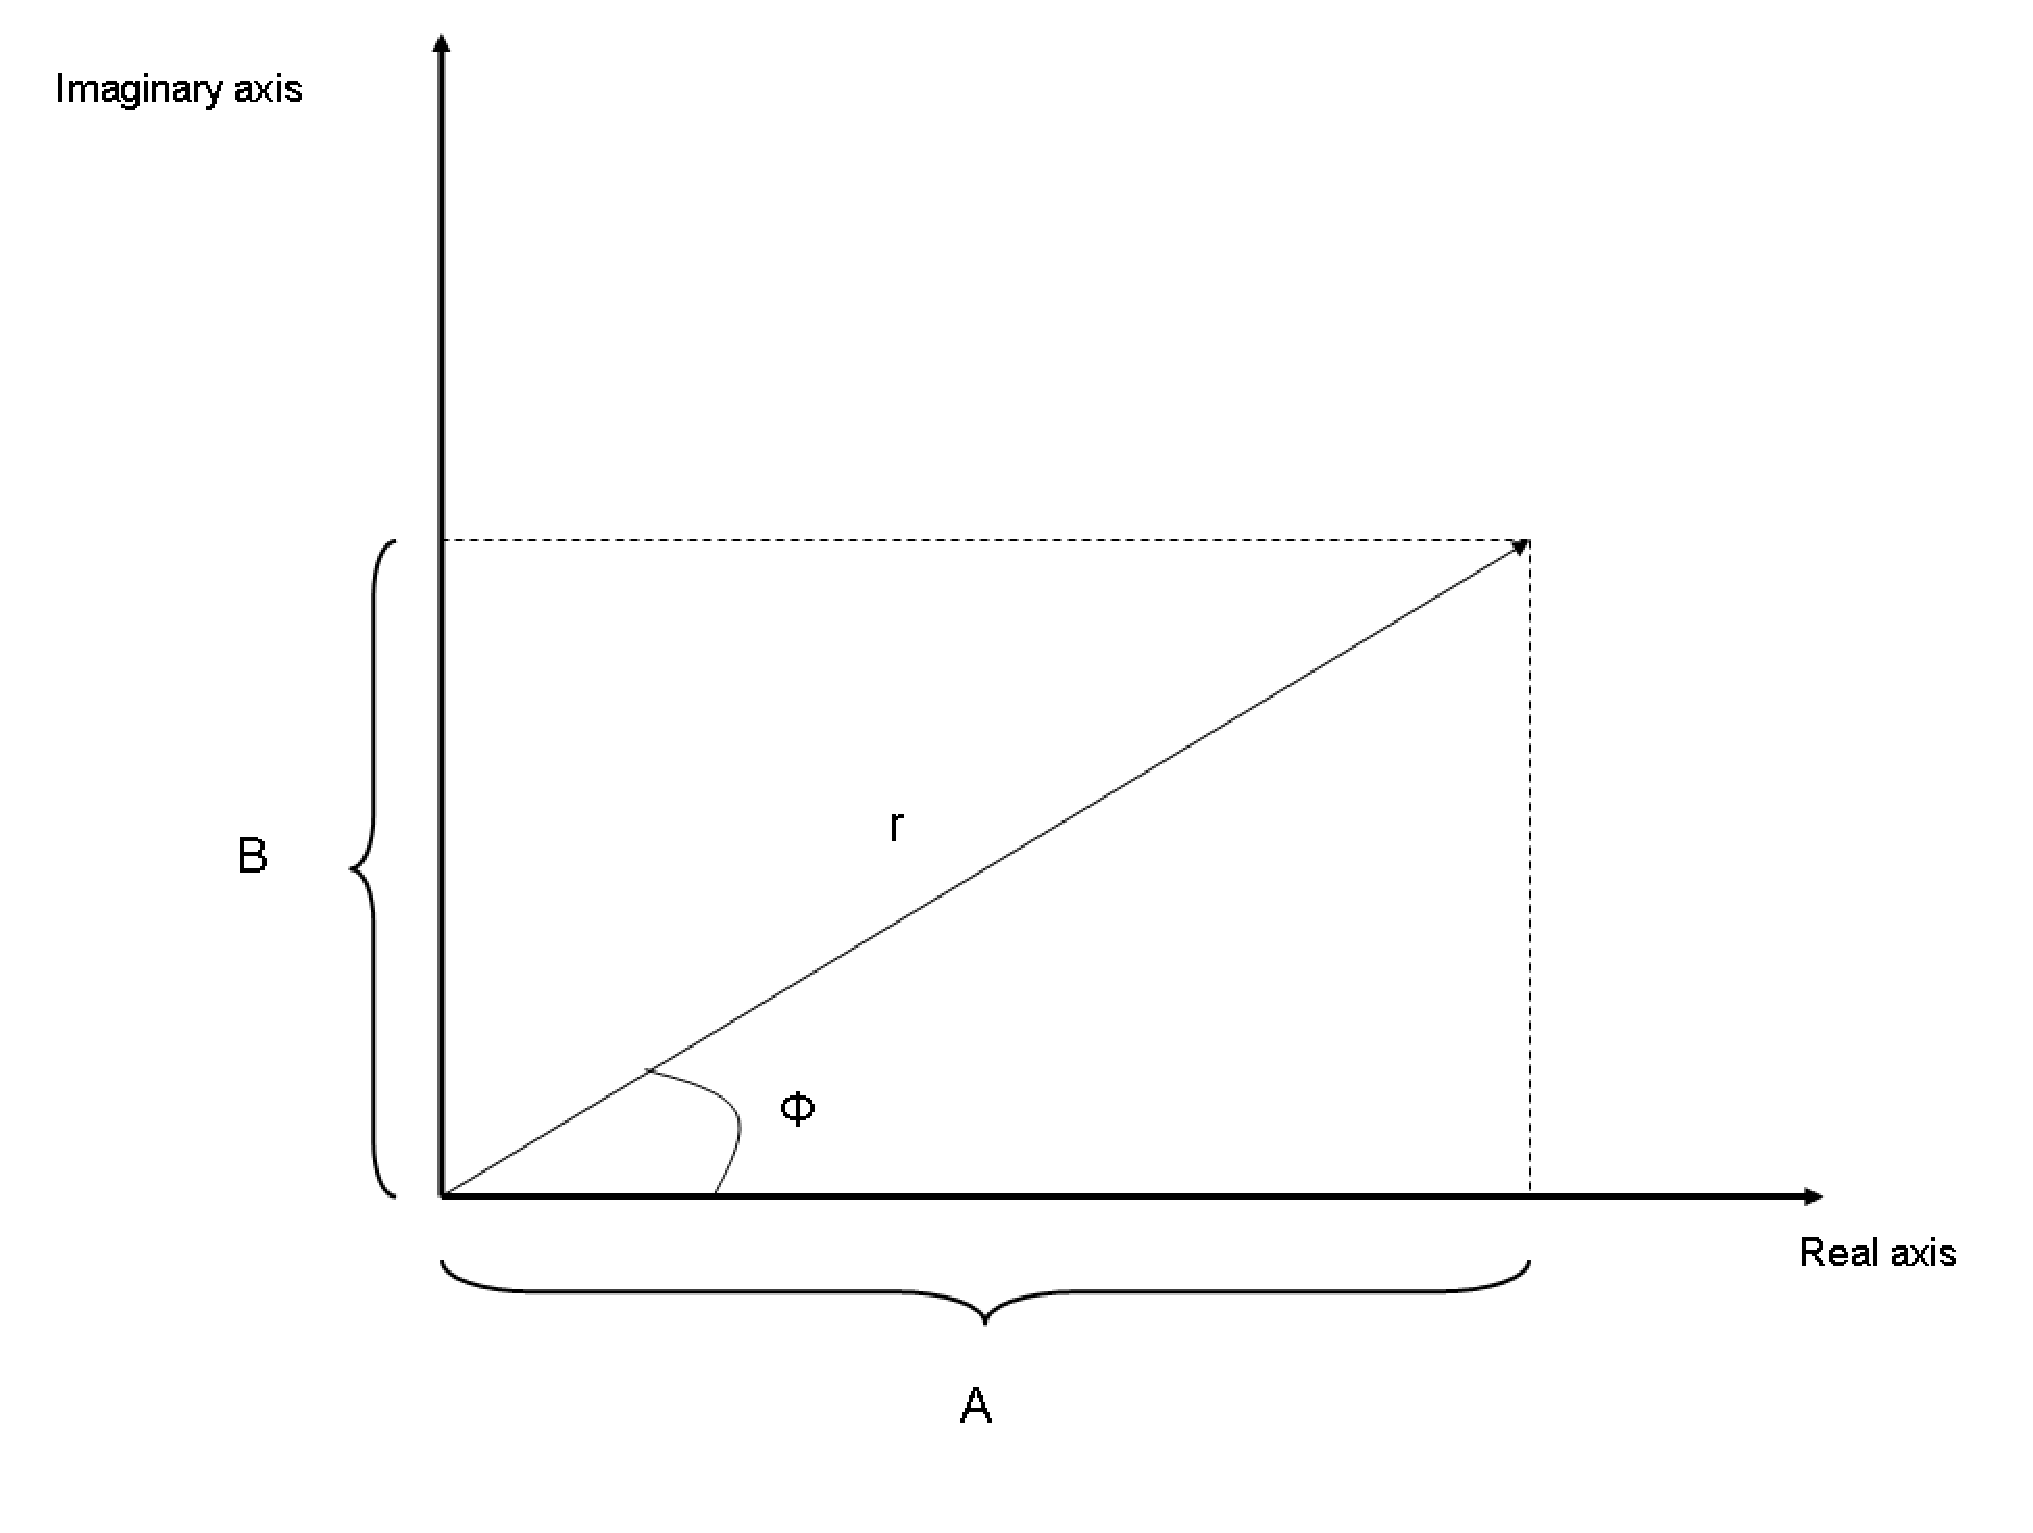
\includegraphics[width=.5\textwidth]{figs_steph/FigurePhase}
\end{center}

\end{itemize}


An $m^{th}-$order linear homogeneous equation with constant coefficients is defined as
\begin{equation}\label{eq:LinH}
a_0x_{t+m}+a_1x_{t+m-1}+\dots + a_m x_{t}=0
\end{equation}
Solutions are composed of linear superpositions of $m$ solutions of the form 
$x_t=\lambda ^t$, $\lambda \not = 0$
where $\lambda$ are obtained by finding the roots (eigenvalues) of the characteristic equation
$$a_0\lambda^{m}+a_1\lambda^{m-1}+\dots + a_m =0.$$
The characteristic equation has $m$ eigenvalues: $\lambda _i,$ $i=1,\dots, m$. 

If eigenvalues are all real and distinct, the general solution takes the form
$$x_t=c_1\lambda_1^t+\dots +c_m\lambda_m^t$$
where $c_i$, $i=1,\dots ,m$ are arbitrary.

For the other cases, general solutions depend on the existence of repeated or complex conjugate eigenvalues. If there is a real eigenvalue $\lambda _1$ of multiplicity $k$, then $k$ linearly independent solutions can be formed by multiplying by powers of $t$:
$$\lambda_1 ^t, t \lambda_1 ^t, t^2\lambda_1 ^t, \dots , t^{k-1}\lambda_1 ^t.$$
If there are complex eigenvalues $\lambda _{1,2}=r(\cos \phi \pm i \sin \phi)$ of multiplicty $k$, then there are $2k$ linearly independent solutions:
$$r^t\cos(t\phi),r^t\sin (t\phi),tr^t\cos(t\phi),tr^t\sin (t\phi),\dots,t^{k-1}r^t\cos(t\phi),t^{k-1}r^t\sin (t\phi)$$




\subsection{Second-order and higher-order linear nonhomogeneous equations}
An $m^{th}-$order linear nonhomogeneous equation  is defined as
\begin{equation}\label{eq:LinNonH}
a_0x_{t+m}+a_1x_{t+m-1}+\dots + a_m x_{t}=b(t)
\end{equation}

\begin{theorem}
The general solution of \eqref{eq:LinNonH} is
$$x_t=x_t^p+\sum_{i=1}^m a_i x_t^i$$
where $x_t^p$ is a particular solution of the nonhomogeneous equation and $\{x_t^1, x_t^2,\dots, x_t^k\}$ is a fundamental set of solutions of $m^{th}$ homogeneous equation \eqref{eq:LinH}.
\end{theorem}


To find a particular solution of a nonhomogeneous equation, there exist several methods:
\begin{itemize}
\item {\bf Method of undetermined coefficient}: making a guess as to the form of the particular solution, and then substituting this function in the difference equation. This method works if the nonhomogeneous term $b(t)$ is a linear combination or product of terms having one of the forms
$$a^t, \quad \cos(ct), \quad  \sin(ct), \quad t^k.$$
See Table \ref{Table1}.
\item {\bf Method of variation of constants}
\end{itemize}

\begin{table}
\begin{tabular}{c|p{7cm}}
$b(t)$ & $x_t^p$
\\\hline
$a^t$ & $c_1 a^t$\\
$t^k$ & $c_0+c_1t+c_2t^2+\dots+c_k t^k$\\
$t^ka^t$ & $c_0a^t+c_1ta^t+c_2t^2a^t+\dots+c_k t^ka^t$\\
$\sin(ct),\cos(ct)$ & $c_1\sin(ct)+c_2\cos(ct)$\\
$a^t\sin(ct),a^t\cos(ct)$ & $(c_1\sin(ct)+c_2\cos(ct))a^t$\\
$a^tt^k\sin(ct),a^tt^k\cos(ct)$ & $(d_0+d_1t+d_2t^2+\dots+d_k t^k)\sin(ct)a^t+(c_0+c_1t+c_2t^2+\dots+c_k t^k)\cos(ct)a^t$\\
\end{tabular}
\label{Table1}
\caption{Particular solutions}
\end{table}


\subsection{Qualitative analysis}
What is the long-term behaviour of the solutions?

For linear difference equations, the asymptotic behavior depends on the eigenvalues: real and complex and the magnitude of eigenvalues.

\begin{definition}
Magnitude of an eigenvalue:
\begin{itemize}
\item If $\lambda=A$ is real, $|\lambda|=|A|$.
\item If $\lambda=A+iB$ is complex, $|\lambda|=|A+iB|=\sqrt{A^2+B^2}$.
\end{itemize}
\end{definition}


\begin{definition}
An eigenvalue $\lambda _i$ such that
$$|\lambda _i|\geq |\lambda _j|$$
for all $j\not =i$ is called the dominant eigenvalue. If the inequality is strict, then $\lambda _i$ is a strictly dominant eigenvalue.
\end{definition}

%\begin{itemize}
%\end{itemize}

Let the general solution of \eqref{eq:LinH} be
$$x_t=\sum_{i=1}^m c_i \lambda_i^t$$

The limiting behavior of the general solution is determined by the behavior of the dominant solution (correspondant to the dominant eigenvalue). Let $\lambda _1$ be the strictly dominant eigenvalue ($|\lambda _1|> |\lambda _j|$ for all $j\not =1$) then
$$x_t=\lambda _1^t\left[ c_1+\sum_{i=2}^m c_i\left ( \frac{\lambda_i}{\lambda_1}\right )^t\right ]$$
Since $\left |\frac{\lambda _i}{\lambda _1}\right |<1$, for all $i\not =1$, then $\left ( \frac{\lambda_i}{\lambda_1}\right )^t\rightarrow 0$ as $t\rightarrow +\infty$. Then $$\lim _{t\rightarrow +\infty }x_t=\lim _{t\rightarrow +\infty }c_1\lambda _1^t.$$
Depending on the value of $\lambda _1$ there are different situations
\begin{itemize}
\item $\lambda _1$ Real
\begin{itemize}
\item $\lambda _1 >1:$ $\lim _{t\rightarrow +\infty }c_1\lambda _1^t=\infty$ (monotonically diverge $\Rightarrow$ unstable system)
\item $\lambda _1 =1:$ constant
\item $0 <\lambda _1 <1:$ $\lim _{t\rightarrow +\infty }c_1\lambda _1^t=0$ (monotonically decreasing to 0 $\Rightarrow$ stable system)
\item $-1 <\lambda _1 <0:$ $\lim _{t\rightarrow +\infty }c_1\lambda _1^t=0$ (oscillating around zero and converging to 0 $\Rightarrow$ stable system)
\item $\lambda _1 =-1:$ system oscillating between two values $c_1$ and $-c_1$
\item $\lambda _1 <-1:$ system is oscillating but increasing in magnitude (unstable system)
\end{itemize}
\item $\lambda _1$ Complex
\begin{itemize}
\item $|\lambda _1|>1$: system oscillates but increases in magnitude (unstable system)
\item $|\lambda _1|=1$: system oscillates but constant magnitude 
\item $|\lambda _1|<1$: system oscillates but converges to 0 (stable system)
\end{itemize}
\end{itemize}

Magnitude of eigenvalues determine whether solutions are unbounded or bounded. The nature, real or complex determine whether solutions oscillate, or not.

In the case of a nonhomogeneous difference equation with a constant nonhomogeneous term, if the system converges, it will converge to the equilibrium point $x^*$ (not to $0$ as previously).



\section{First-order Linear system}
A higher-order linear difference equation can be converted to a first-order linear system.


An $m^{th}-$order linear nonhomogeneous equation is 
$$
a_0x_{t+m}+a_1x_{t+m-1}+\dots + a_m x_{t}=b(t)
$$
for convenience $x_t$ is now denoted $x(t)$. Let $Y(t)$ be a $m-$vector  $Y(t)=(y_1(t),y_2(t),\dots, y_m(t))$ that satisfies
\begin{equation*}
\begin{array}{cc}
y_1(t)=&x(t)\\
y_2(t)=&x(t+1)\\
y_3(t)=&x(t+2)\\
\vdots &\\
y_{m}(t)=&x(t+m-1)
\end{array}
\end{equation*}
the first element $y_1(t)$ is the solution $x(t)$. Hence a first-order difference equation in $y$ is 
\begin{equation*}
\begin{array}{cl}
y_1(t+1)=&y_2(t)\\
y_2(t+1)=&y_3(t)\\
y_3(t+1)=&y_4(t)\\
\vdots &\\
y_{m-1}(t+1)=&y_{m}(t)\\
y_{m}(t+1)=&-a_1 y_m(t)-\dots -a_{m-1}y_2(t)- a_m y_1(t)+b(t)
\end{array}
\end{equation*}
In matrix form,
$$Y(t+1)=AY(t)+B$$
where
$$A=\left (
\begin{array}{ccccc}
0 & 1 & 0 & \hdots & 0\\
0 & 0 & 1 & \hdots & 0\\
\vdots & \vdots & \vdots & \ddots & \vdots\\
0 & 0 & 0 & \hdots & 1\\
-a_{m} & -a_{m-1} & -a_{m-2} & \hdots & -a_{1}
\end{array}
\right), \quad B=\left ( \begin{array}{c}
0\\
0\\
\vdots\\
0\\
b(t)
\end{array}
\right).
$$ 
The matrix $A$ has 1's along the superdiagonal and has the coefficients of the higher-order difference equation $-a_i$ (but the signs are reversed) along the last row. Matrix is called the {\bf companion matrix} of the $m^{th}-$order difference equation.


A solution to a first-order linear difference system $X(t+1)=AX(t)+B$ is the superposition of two solutions: the general solution $X_h$ to the homogeneous system $X_h(t+1)=AX_h(t)$ and a particular solution $X_p$ to the nonhomogeneous system $X_p(t+1)=AX_p(t)+B$. The general solution to the nonhomogeneous system is $$X(t)=X_h(t)+X_p(t).$$


The homogeneous system has $m-$linearly independent solutions: there are some direct and indirect methods to find these linearly independent solutions.

{\bf Indirect methods} use the fact that the solution can be expressed as $X(t)=A^tX(0). $ In \cite{Elaydi1998}, methods to compute $A^t$ are presented, then the general solution can be known.

{\bf Direct method} to solve $X(t+1)=AX(t)$ where $A=(a_{ij})$ is an $m\times m$ constant matrix:
Assume that a solution has the following form $X(t)=\lambda ^t V$ where $V$ is an nonzero $m-$column vector and $\lambda$ is a constant. Substituting $\lambda ^t V$ into the linear system gives
$$\lambda ^{t+1} V=A\lambda ^t V,$$
then
\begin{equation}(A - \lambda I) V=\mathbf{0}\label{eq:Cha}\end{equation}
where $I$ is the $m\times m$ identity matrix and $\mathbf{0}$ is the zero vector. The zero solution $V=0$ is the trivial solution; and \eqref{eq:Cha} has an unique solution if $\det(A - \lambda I)\not =0$. Hence, nonzero solutions $V$ are obtained if and only if $(A - \lambda I) $ is singular if and only if 
\begin{equation}\det(A - \lambda I) =0.\label{eq:Charac}\end{equation}

Equation \eqref{eq:Charac} is referred as the {\bf characteristic equation of matrix} $A$. The $m$ solutions $\lambda_i$, $i=1,\dots, m$ of \eqref{eq:Charac} are called the {\bf eigenvalues} of the matrix $A$. The nonzero solutions $V_i$ are the {\bf eigenvectors} corresponding to the eigenvalue $\lambda_i$ that are found by solving $(A - \lambda_i I) V_i=\mathbf{0}$.

Then the general solution is a linear combination of $m$ linearly independent solutions $X_i=\lambda _i ^t V_i$, $i=1,\dots, m$:
\begin{equation}X(t)=\sum_{i=1}^m c_i\lambda _i ^t V_i\label{eq:solFirstSyst}\end{equation}
where $c_i$ are arbitrary constants.

The asymptotic behavior of the solution \eqref{eq:solFirstSyst} does not require the knowlegde of the eigenvectors. The asymptotic behavior is determined by the eigenvalues and their magnitude.

\begin{definition}
The spectral radius of matrix $A$ is denoted $\rho(A)$ and is defined as
$$\rho(A)=\max_{i\in \{1,2,\dots,m\}}|\lambda_i|$$
\end{definition}


\begin{theorem}\label{Theo:NormRho}
Let $A$ be a $k\times k$ matrix
$$\rho(A)\leq \| A\| $$
\end{theorem}



$ \| A\|_1=\max_{1\leq j\leq k}\sum_{i=1}^k|a_{ij}|$ (Sum over columns)

$ \| A\|_{\infty}=\max_{1\leq i\leq k}\sum_{j=1}^k|a_{ij}|$ (Sum over rows)

$ \| A\|_2=[\rho(A^TA)]^{1/2}$


\begin{theorem}\label{Theorem:MatrixConverg}
Let $A$ be a constant $m \times m$ matrix. Then the spectral radius of $A$ satisfies $\rho(A)<1$ if and only if $$\lim_{t\rightarrow + \infty}A^t=\mathbf{0}$$
\end{theorem}

As the solution of $X(t+1)=AX(t)$ is $X(t)=A^tX(0)$, $\lim_{t\rightarrow + \infty} X(t)=0$ when $\rho(A)<1$.

\subsection{Nonnegative matrices}
\begin{definition}
A matrix $A$ whose entries are nonnegative is called a nonnegative matrix, denoted $A\geq 0$.
\end{definition}


\begin{definition}
A matrix $A$ whose entries are positive is called a positive matrix, denoted $A> 0$.
\end{definition}


\begin{definition}
A square $m\times m$  matrix $A=a_{ij}$ is said to be reductible if the index set $1,2, \dots, m$ can be split into two nonempty complementary sets $S_1$ and $S_2$: $S_1=\{i_1,\dots , i_{\mu}\}$ and $S_2=\{k_1,\dots , k_{\varepsilon}\}$ where $m=\mu+\varepsilon$ such that
$$a_{i_\alpha k_{\beta}}=0 \quad (\alpha = 1,2,\dots , \mu; \beta = 1,2, \dots, \varepsilon).$$
Otherwise, matrix $A$ is irreductible.
\end{definition}


\begin{definition}
If there exits a directed path from node $i$ to $j$ for every node $i$ and $j$ in the digraph, then the digraph is said to be strongly connected.
\end{definition}

\begin{theorem}
The digraph of matrix $A$ is strongly connected if and only if $A$ is irreductible.
\end{theorem}


\begin{theorem}(Frobenius Theorem)
An irreductible, nonnegative matrix $A$ always has a positive eigenvalues $\lambda$ that is a simple root (multiplicity one) of the characteristic equation. The value of $\lambda$ is greater than or equal to the magnitude of all of the other eigenvalues. To the eignevalue $\lambda$ there corresponds an eigenvector with positive coordinates.
\end{theorem}


\begin{theorem}(Perron Theorem)
A positive matrix $A$ always has a real, positive eigenvalue $\lambda$ that is a simple root of the characteristic equation and exceeds the magnitude of all of the other eigenvalues
$$|\lambda _i|<|\lambda|,\quad \forall i.$$
To the eigenvalue $\lambda$ there corresponds an eigenvector with positive coordinates.
\end{theorem}


\begin{definition}
If an irreductible, nonnegative matrix $A$ has $h$ eigenvalues $\lambda _1, \lambda _2, \dots \lambda _h$ of maximum modulus ($|\lambda _1 |= |\lambda _i|, i=1,2,\dots ,h $), then $A$ is called primitive if $h=1$ and imprimitive if $h>1$. The value of $h$ is called the index of imprimitivity.
\end{definition}

The index of imprimitivity is the number of eigenvalues of matrix $A$ with maximum modulus (with magnitude equal to $\rho(A)$).

\begin{theorem}
A nonnegative matrix $A$ is primitive if and only if some power of $A$ is positive (i.e. $A^p>0$ for some integer $p\geq 1$).
\end{theorem}

\begin{theorem}\cite{Berman1994}
A irreductible matrix is primitive if its trace if positive. 
\end{theorem}


\begin{theorem}(Perron-Frobenius Theorem)
If $M$ is a nonnegative primitive matrix, then:
\begin{itemize}
\item $M$ has a positive eigenvalue $\lambda_1$ of maximum modulus.
\item $\lambda_1$ is a simple root of the characteristic polynomial.
\item for every other eigenvalue $\lambda _i$, $\lambda_1>\lambda_i$ (it is strictly dominant)
\item $$\min_{i}\sum_j m_{ij}\leq \lambda _1 \leq \max_{i}\sum_j m_{ij} $$
$$\min_{j}\sum_i m_{ij}\leq \lambda _1 \leq \max_{j}\sum_i m_{ij} $$
\item the row and column eigenvectors associated with $\lambda_1$ are strictly positive.
\item the sequence $M^t$ is asymptotically one-dimensional, its columns converge to the column eigenvector associated with $\lambda_1$; and its rows converges to the row eigenvector associated with $\lambda_1$.
\end{itemize}
\end{theorem}

\subsubsection{Leslie matrix model}
Structured population models are used when the population can be organized or divided into various parts.


Structured models: the structuring variable can be age, stage or size
\begin{itemize}
\item age-structured model:  population is subdivided into age group (for human population, age group may be 5 year length, 0-5, 5-10, $\dots$).
\item stage-structured model: population is organized into developmental stage (juveniles and adult) (or for insects: egg, larva, pupa, adult).
\item size-structured  model: individuals in population are grouped according to size (length or weight)
\end{itemize}
The dynamic interactions among the stages, ages or sizes determine how the population structure changes over the time. Other structuring variables can be taken into account: sex and space.


The Leslie Matrix (also called the Leslie Model) describes the growth of populations with structure (and their projected age distribution); the population is closed to migration and only one sex, usually the female, is considered.


Assume the population is closed to migration and only the females are modeled. Males are presented, but are not specifically modeled (when the sex ratio of males to females is $a/b$ and the survival rate per age group is the same for males and females, then the number of males equals the number of females times $a/b$). 


Let the total number of age groups is $m$ ($m$ the last reproductive age). During the interval of time $t$ and $t+1$ individuals age from $i$ to $i+1$: time interval coincides with the age interval.
\begin{itemize}
\item $x_i(t)$ number of females in the $i^{th}$ age group at time $t$.
\item $b_i$ average number of newborn females produced by one females in the $i^{th}$ age group that survive through the time interval in which they were born, $b_i\geq 0$
\item $s_i$ fraction of the $i^{th}$ age group that lives  to the $(i+1)st$ age, $0<s_i\leq 1$
\end{itemize}
\begin{center}
\begin{figure}
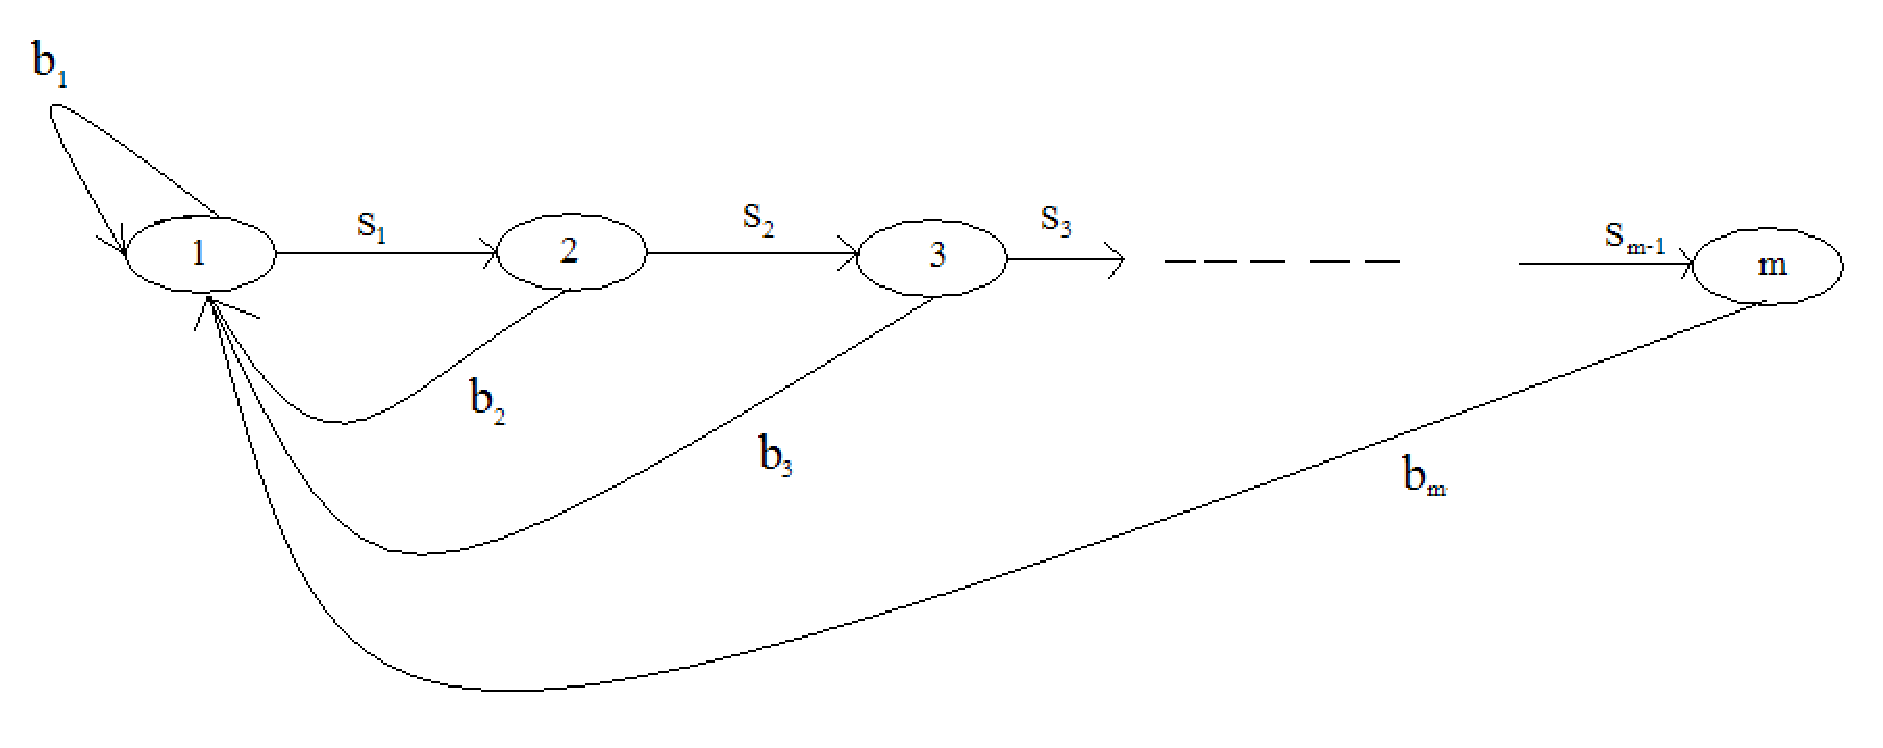
\includegraphics[width=1\textwidth]{figs_steph/LesliePattern}
\caption{Life cycle graph of the Leslie matrix on $m$ age classes: each node represents each age group $x_i$, and arcs represent relation between two groups. An arrow connects the node $j$ to $i$ if the $ij^{th}$ element in the Leslie matrix $L$ is nonzero.}
\end{figure}
\end{center}

\begin{subequations} 
\begin{align}
x_{1}(t+1)=& b_1 x_1(t)+b_2x_2(t)+b_3x_3(t)+\dots b_mx_m(t)\label{eq:Leslie1}\\
x_{2}(t+1)=&s_1 x_1(t)& \label{eq:Leslie2}\\
x_{3}(t+1)=&s_2 x_2(t)& \label{eq:Leslie3}\\
\vdots &\\
x_{m}(t+1)=&s_{m-1} x_{m-1}(t)& \label{eq:Leslie3}\\
\end{align}   
\end{subequations} 
Using matrix notation,
\begin{equation}
X(t+1)=\left (
\begin{array}{c}
x_1(t+1)\\
x_2(t+1)\\
x_3(t+1)\\
\vdots\\
x_m(t+1)
\end{array}
\right )
=
\left(
\begin{array}{ccccc}
b_1 & b_2 & \hdots & b_{m-1} & b_m\\
s_1 & 0  & \hdots & 0 & 0\\
0 & s_2  & \hdots & 0 & 0\\
\vdots & \vdots & \ddots & \vdots & \vdots \\
0 &0 &\hdots & s_{m-1} &0
\end{array}
\right)
\left (
\begin{array}{c}
x_1(t)\\
x_2(t)\\
x_3(t)\\
\vdots\\
x_m(t)
\end{array}
\right )=LX(t)
\end{equation}
where $L$ is called the Leslie matrix: fertilities or fecundities on the first row and survival probabilities on the subdiagonal. All other entries in the Leslie matrix are zero.



$$X(1)=LX(0)$$
$$X(2)=LX(1)=L\left(LX(0)\right)=L^2X(0)$$
In general
$$X(t)=L^tX(0)$$







\begin{definition}
A Leslie matrix is a nonnegative matrix.
\end{definition}




A necessary condition for a Leslie matrix to be irreductible is $b_m\not =0$.


Frobenius Theorem gives sufficient conditions that guarantees the Leslie matrix has one positive strictly dominant eigenvalue.


If the Leslie matrix satisfies $L^p>0$ for some positive integer $p$, then $L$ is primitive. Then, the Frobenius Theorem states that in this case L has a unique strictly dominant eigenvalue $\lambda _1$ satisfying $|\lambda _1|>|\lambda _i|$, for $j\not =1$, that is positive. Associated with the strictly dominant eigenvalue $\lambda _1$ is a positive eigenvector $V_1$, that is referred to as a stable age distribution.


Assume matrix $L$ is irreductible and primitive and $m$ eigenvectors form a linearly independent set; then the solution to
$$X(t+1)=LX(t)$$
can be written
$$X(t)=L^tX(0)=\sum_{i=1}^m c_i \lambda _i ^t V_i$$
where $\lambda _1$ is the strictly dominant eigenvalue. Dividing the solution by $\lambda _1^t$ gives
$$\frac{X(t)}{\lambda _1^t}=\frac{L^tX(0)}{\lambda _1^t}=c_1 V_1 + \frac{c_2 \lambda _2 ^t}{\lambda _1^t} V_2+\dots + \frac{c_m \lambda _m ^t}{\lambda _1^t} V_m $$
As $|\lambda _i/\lambda_1|<1$, $(\lambda _i/\lambda_1)^t\rightarrow 0$ as $t\rightarrow +\infty$. Thus
$$\lim_{t\rightarrow +\infty} \frac{X(t)}{\lambda _1^t}=\lim_{t\rightarrow +\infty}  \frac{L^tX(0)}{\lambda _1^t}=c_1V_1 .$$
Hence after many generations, $X(t)=L^tX(0)=c_1\lambda _1^tV_1$. The population size either increasing ($\lambda _1 >1$) or decreasing ($\lambda _1 <1$) geometrically as $t$ goes larger.

The population distribution $X(t)/\lambda _1 ^t$ approaches a constant multiple of the eigenvector $V_1$; thus $V_1$ is referred to as a stable age distribution. It means that for large values of time, the age distribution vector is a scalar multiple of the eigenvector associated with the largest eigenvalue of the matrix. Consequently the proportion of females in each of the age classes becomes constant, these limiting proportions can be determined from the eigenvector $V_1$.

An explicit expression for $V_1$ in the case of a Leslie matrix is \cite{Pielou1977}
\begin{equation}
\label{eq:Eigenvector}
V_1=\left (\begin{array}{c}
1\\
\frac{s_1}{\lambda _1}\\
\vdots\\
\frac{s_1s_2\dots s_{m-2}}{\lambda_1^{m-2}}\\
\frac{s_1s_2\dots s_{m-1}}{\lambda_1^{m-1}}
\end{array}\right )
\end{equation}


The characteristic equation for the Leslie matrix satisfies $\det(L-\lambda I)=0$ or
$$\det 
\left(
\begin{array}{ccccc}
b_1-\lambda & b_2 & \hdots & b_{m-1} & b_m\\
s_1 & -\lambda  & \hdots & 0 & 0\\
0 & s_2  & \hdots & 0 & 0\\
\vdots & \vdots & \ddots & \vdots & \vdots \\
0 &0 &\hdots & s_{m-1} &-\lambda
\end{array}
\right)=0$$
or
$$p(\lambda)=\lambda ^m-b_1 \lambda^{m-1}-b_2s_1 \lambda^{m-2}- b_3s_1 s_2 \lambda^{m-3}-\dots - b_m s_1s_2 s_3\dots s_{m-1}=0 $$
From Descarte's Rule, since there is only one change in sign in the polynomial, $p(\lambda)$ has one positive real root, that is the dominant eigenvalue $\lambda _1$.

How is the dominant eigenvalue $\lambda _1$: $\lambda _1 >1$ or $\lambda _1 <1$?
\begin{itemize}
\item $\lim _{\lambda \rightarrow \infty}p(\lambda)=\infty$
\item $p(0)<0$
\item $p(\lambda)$ crosses the positive $\lambda-$axis only once at $\lambda_1$
\end{itemize}
then 
\begin{itemize}
\item $\lambda _1 >1$ $\Leftrightarrow$ $p(1)<0$
\item $\lambda _1 <1$ $\Leftrightarrow$ $p(1)>0$
\end{itemize}
where $p(1)=1-b_1 -b_2s_1 - b_3s_1 s_2 -\dots - b_m s_1s_2 s_3\dots s_{m-1}$, and $p(1)=1-R_0$.
Hence
\begin{itemize}
\item $\lambda _1 >1$ $\Leftrightarrow$ $1<R_0$
\item $\lambda _1 <1$ $\Leftrightarrow$ $1>R_0$
\end{itemize}

\begin{definition}
The reproductive number $R_0$ is the average number of offspring produced by an
individual in its lifetime:
$$R_0=b_1+b_2s_1+b_3s_1s_2+\dots+b_ms_1s_2\dots s_{m-1}$$
where each term represent the average
number of offsprings produced by individuals of age $i$.
\begin{itemize}
\item $R_0 < 1$ individuals not fully replacing themselves, population shrinking
\item $R_0 = 1$ individual exactly replacing themselves, population size stable
\item $R_0 > 1$ individuals more than replacing themselves, population growing
\end{itemize}
\end{definition}


\begin{theorem}
Assume the Leslie matrix $L$ defined as
$$X(t+1)=\left (
\begin{array}{c}
x_1(t+1)\\
x_2(t+1)\\
x_3(t+1)\\
\vdots\\
x_m(t+1)
\end{array}
\right )
=
\left(
\begin{array}{ccccc}
b_1 & b_2 & \hdots & b_{m-1} & b_m\\
s_1 & 0  & \hdots & 0 & 0\\
0 & s_2  & \hdots & 0 & 0\\
\vdots & \vdots & \ddots & \vdots & \vdots \\
0 &0 &\hdots & s_{m-1} &0
\end{array}
\right)
\left (
\begin{array}{c}
x_1(t)\\
x_2(t)\\
x_3(t)\\
\vdots\\
x_m(t)
\end{array}
\right )=LX(t)
$$
is irreductible and primitive. The characteristic polynomial of $L$ i given by
$$p(\lambda)=\lambda ^m-b_1 \lambda^{m-1}-b_2s_1 \lambda^{m-2}- b_3s_1 s_2 \lambda^{m-3}-\dots - b_m s_1s_2 s_3\dots s_{m-1}=0 .$$
Matrix $L$ has a strictly dominant eigenvalue $\lambda _1>0$ satisfying the following relationships:
\begin{itemize}
\item $\lambda _1 =1$ if and only if $R_0=1$,
\item $\lambda _1 <1$ if and only if $R_0<1$,
\item $\lambda _1 >1$ if and only if $R_0>1$,
\end{itemize}
where $R_0$ is the inherent reproductive number defined by
$$R_0=b_1+b_2s_1+b_3s_1s_2+\dots+b_ms_1s_2\dots s_{m-1}.$$
In addition the stable age distribution $V_1$ satisfies
$$V_1=\left (\begin{array}{c}
1\\
\frac{s_1}{\lambda _1}\\
\vdots\\
\frac{s_1s_2\dots s_{m-2}}{\lambda_1^{m-2}}\\
\frac{s_1s_2\dots s_{m-1}}{\lambda_1^{m-1}}
\end{array}\right ).
$$
\end{theorem}


\subsubsection{Markov chains}
Suppose that we conduct some experiment with a set of $k$ states $S=\{s_1,\dots, s_k\}$. The experiment is repeated such that the probability $p_{ij}$ of the state $s_i$, $1\leq i\leq k$, occuring on the $(n+1)^{th}$ repetition depends only on the state $s_j$ occurring on the $n^{th}$ repetition of the experiment. The system has no memory: the future state depends only on the present state. The probability of $s_i$ ocurring on the next repetition, given that $s_j$ occurred on the last repetition is
$$p_{ij}=p(s_i|s_j).$$
Given that $s_j$ has occured in the last repetition, one of $s_1$, $s_2$, $\dots, s_k$ must occur in the next repetition, then
$$p_{1j}+p_{2j}+p_{3j}+\dots+p_{kj}=1, \quad 1\leq j\leq k.$$
Let $p_i(n)$ be the probability that the state $s_i$ will occur on the $n^{th}$ repetition of the experiment, $1\leq i\leq k$. Since one the states $s_i$ must occur on the $n^{th}$ repetition it follows that
$$p_1(n)+p_2(n)+\dots+p_k(n)=1.$$
The probability that the state $s_i$, $1\leq i\leq k$, occurs on the $(n+1)^{th}$ repetition of the experiment is $p_i(n+1)$. There are $k$ way to obtain this. The first case is where repetition $n$ gives us $s_1$, and the repetition $(n+1)$ produces $s_i$. Since the probability of getting $s_1$ on the $n^{th}$ repetition is $p_1(n)$, and the probability of having $s_i$ after $s_1$ is $p_{i1}$, it follows (by multiplication principle) that the probability of the first case occurring is $p_{i1}p_1(n)$. The second case is where we get $s_2$ on the repetition $n$ and $s_i$ on repetition $(n+1)$. The probability of the occurrence of the second case is $p_{i2}p_2(n)$. Similarly for $3,\dots k$, hence

$$
\begin{array}{ll}
p_1(n+1)=& p_{11}p_1(n)+p_{12}p_2(n)+p_{13}p_3(n)+\dots+p_{1k}p_k(n)\\
p_2(n+1)=& p_{21}p_1(n)+p_{22}p_2(n)+p_{23}p_3(n)+\dots+p_{2k}p_k(n)\\
\vdots =&\\
p_k(n+1)=& p_{k1}p_1(n)+p_{k2}p_2(n)+p_{k3}p_3(n)+\dots+p_{kk}p_k(n)
\end{array}
$$
in matrix form
\begin{equation}
p(n+1)=S p(n), \quad n=1,2,3,\dots
\end{equation}
where $p(n)=(p_1(n),p_{2}(n),\dots , p_k(n))^T$ is the probability vector and $S=(p_{ij})$ is a $k\times k$ transition matrix.

\begin{definition}
The nonnegative $k\times k$ matrix $A$ is said to be stochastic if $\sum_{i=1}^ka_{ij}=1$ for all $j=1,2,\dots, k$.
\end{definition}

\begin{definition}
A regular Markov chain is one in which $S^p$ is positive for some positive integer $p$.
\end{definition}

From Theorem \ref{Theo:NormRho}
$$\rho(S)\leq \| S\| _1 =1$$
then $|\lambda|\leq 1$ for all eigenvalues of a stochastic matrix. Furthermore, if $S$ is a stochastic matrix $\lambda =1$ is an eigenvalue of $S$; hence $\rho(S)=1$ and the dominant eigenvalue $\lambda _1 =1$. Then
$$\lim_{n\rightarrow +\infty}p(n)=\lim_{n\rightarrow +\infty}S^np(0)=cV_1$$
where $V_1=(v_1,v_2,\dots ,v_k)$ is the eigenvector that corresponds to the dominant eigenvalue $\lambda _1 =1$.

Since $p(n)=(p_1(n),p_2(n),\dots , p_k(n))^T$, we have $\sum_{i=1}^k p_i(n)=1$, it follows that
$$cv_1+cv_2+\dots cv_k=1.$$
Therefore
$$c=\frac{1}{v_1+v_2+\dots+v_k}.$$


\begin{definition}
A state $s_i$ in a Markov chain is said to be absorbing if whenever it occurs on the $n^{th}$ generation of the experiment, it then occurs on every subsequent repetition. In other word, if for some $p_{ii}=1$ then $p_{ij}=0$ for $i\not =j$.
\end{definition}

\begin{definition}
A Markov chain is said to be absorbing if it has at least one absorbing state, and if from every state it is possible to go to an absorbing state.
\end{definition}

In an absorbing Markov chain, a state that is not absorbing is called transient.


\section{Examples}
\subsection{Bacteria population}
E. coli are able to divide every 20 minutes under optimal conditions. Describe the temporal evolution of a colony of E. coli.


\begin{definition}
Cell division is the process by which a cell, called the parent cell, divides into two cells, called daughter cells. Cell division is usually a small segment of a larger cell cycle.
\begin{itemize}
\item Prokaryotic cells: binary fission
\item Eukaryotic cells: mitosis+cytokinesis
\end{itemize}
\end{definition}

\begin{definition}
Binary fission: The prokaryotic chromosome is a single DNA molecule that first replicates, then attaches each copy to a different part of the cell membrane. When the cell begins to pull apart, the replicate and original chromosomes are separated. Following cell splitting (cytokinesis), there are then two cells of identical genetic composition (except for the rare chance of a spontaneous mutation).
\end{definition}
\begin{center}
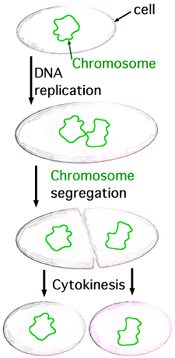
\includegraphics[width=.25\textwidth]{figs_steph/Binary_fission}
\end{center}



\begin{definition}
Mitosis+Cytokinesis: Mitosis is the process by which a cell separates its duplicated genome into two identical halves. It is generally followed immediately by cytokinesis which divides the cytoplasm and cell membrane. This results in two identical daughter cells with a roughly equal distribution of organelles and other cellular components. Mitosis and cytokinesis together is defined as the mitotic (M) phase of the cell cycle, the division of the mother cell into two daughter cells, each the genetic equivalent of the parent cell.
\end{definition}
\begin{center}
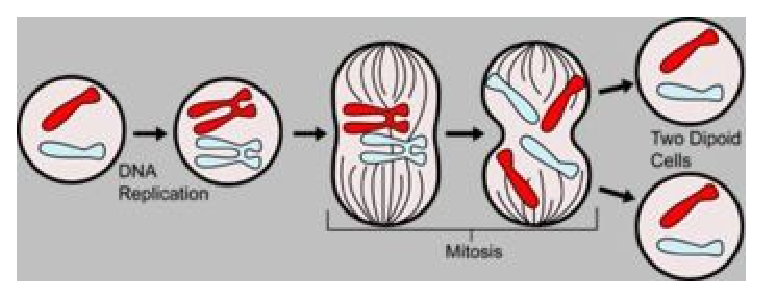
\includegraphics[width=.8\textwidth]{figs_steph/Mitosis}
\end{center}

Organisms that reproduce by binary fission (asexual reproduction) exhibit exponential growth. If organisms (or cells) are synchronized, the formalism of difference equation can be used.

The model (for an unlimited environment) to describe the temporal evolution of the E. Coli colony is expressed as
$$x_{t+1}=2x_t, \quad t=0,1,2,\dots$$
where $x_t$ is the state variable that repressents the number of cells at the generation $t$. If the initial population $x_0$ is known then the solution is unique and is 
$$x_{t}=2^tx_0, \quad t=0,1,2,\dots$$

Asymptotic behavior of the solution:
$$\lim_{t\rightarrow \infty} x_t=\infty$$
as $a=2>1$. 


\begin{quote}
Note: If differential equation formalism was used
$$\frac{dx}{dt}=\frac{1440}{20}x$$
the solution would be $x(t)=x_0e^{\frac{1440}{20}t}$.
\end{quote}

\subsection{Insect populations}
Assume that adult females of a species produce offspring at a fixed period of time each year. A proportion of the offspring (juveniles) survives to adulhood, reproduces, and dies (nonoverlapping of generations). Let
\begin{itemize}
\item $j_t$ number of juveniles in years $t$
\item $a_t$ number of adult females in year $t$
\item $p$ number of juveniles that survive in year $t$
\item $f$ number of offspring produced per female
\item $r$ ratio of females to adults.
\end{itemize}
Using the definition of state variables and parameters given above, the model can be expressed as follows
$$a_{t+1}=prj_t$$
$$j_{t+1}=f a_{t+1}$$
The system can be condensed in an unique equation:
$$j_{t+1}=f prj_t$$
If the initial population $j_0$ of juveniles is known, the solution is unique and is
$$j_t=(f pr)^tj_0 \quad t=0,1,2,\dots$$
The asymptotic behavior of the solution depends on the value of $f pr$:
\begin{itemize}
\item If $f pr<1$ $\lim_{t\rightarrow +\infty} j_t=0$ extinction of the population,
\item If $f pr>1$ $\lim_{t\rightarrow +\infty} j_t=+\infty$ explosion of the population.
\end{itemize}
\subsection{Pharmacology}
A drug is administred once every four hours. Let $D_n$ be the amount of the drug in the blood system at the $n^{th}$ interval.  The body eliminates a certain fraction $p$ of the drug during each time interval. If the amount administred is $D_0$, find $D_n$ and $\lim _{n \rightarrow}D_{n}$.

$$D_{n+1}=D_n-pD_n +D_0=(1-p)D_n +D_0 \quad n=0,1,\dots$$
and the initial condition is $D_0$.

The equilibrium solution is $D^*=\frac{D_0}{p}$ (obtained by solving $D_{n}=(1-p)D_n +D_0$)
 
Using Proposition \ref{Prop:FirstLinNonH} the solution is unique and is
$$D_n=(1-p)^n\left [D_0-\frac{D_0}{p}\right ] +\frac{D_0}{p} \quad n=0,1,2,\quad$$

Limiting behavior is
$$\lim _{n\rightarrow +\infty}D_n=\frac{D_0}{p}$$
as $(1-p)<1$.

\begin{quote}
Note: If differential equation formalism was used
$$\frac{dD}{dt}=-pD +D_0, \quad D(0)=D_0$$
the solution would be $D(t)=\frac{D_0}{p}+(D_0-\frac{D_0}{p})e^{-pt}$.
\end{quote}


\subsection{Propagation of annual plants}
Plants produce seeds at the end of their growth season (August), after which they die. A fraction of these seeds survive the winter, and some of these germinate at the beginning of the season (May), giving rise to the new generation of plants. The fraction that germinates depends on the age of the seeds. 
\begin{itemize}
\item $\gamma$ number of seeds produced per plant in August
\item $\sigma$ fraction of seeds that survive a given winter
\item $\alpha$ fraction of one-year-old seeds that germinate in May
\item $\beta$ fraction of two-year-old seeds that germinate in May
\item Seeds older than two years are no longer viable
\end{itemize}

State variables:
\begin{itemize}
\item $p_n$ number of plants in generation $n$
\item $s_n$ number of new seed in generation $n$
\item $s^1_n$ number of one-year-old seeds in generation $n$
\item $s_{n}^{2}$ number of two-year-old seeds in generation $n$
\end{itemize}
Equations:
\begin{subequations}\label{eq:plant}
\begin{align}
p_n=&\alpha s^1_n+\beta s_{n}^{2}\label{eq:plant1}\\
s_{n}=&\gamma p_{n}\label{eq:plant2}\\
s_n^1=&\sigma s_{n-1}\label{eq:plant3}\\
s_{n}^{2}=&\sigma (1-\alpha)s^1_{n-1}\label{eq:plant4}
\end{align}   
\end{subequations} 
Condensing equations \eqref{eq:plant2}, \eqref{eq:plant3} and \eqref{eq:plant4} we obtain
$$s_n^1=\sigma \gamma p_{n-1}$$
and 
$$s_{n}^{2}=\sigma (1-\alpha)\sigma \gamma p_{n-2}$$
therefore, we can express the model as a system of 3 First-order difference equations
\begin{equation*}
\begin{array}{ll}
p_n=&\alpha s_n+\beta \sigma (1-\alpha)s_{n-1}\\
s_n^1=&\sigma \gamma p_{n-1}\\
s_{n}^{2}=&\sigma (1-\alpha)\sigma \gamma p_{n-2}
\end{array}
\end{equation*}
or as 1 Second-order equation:
\begin{equation}\label{eq:PLANTS}
p_n=\alpha \sigma \gamma p_{n-1}+\beta \sigma (1-\alpha)\sigma \gamma p_{n-2}
\end{equation}

Characteristic equation corresponding to the model \eqref{eq:PLANTS} is
$$\lambda ^2 - \alpha \sigma \gamma \lambda - \beta \sigma^2 (1-\alpha) \gamma=0$$

Eigenvalues are
$$\lambda _{1,2}=\frac{\alpha \sigma \gamma \pm \sqrt{(\alpha \sigma \gamma)^2+4\beta \sigma^2 (1-\alpha) \gamma}}{2}$$

%=\frac{\alpha \sigma \gamma \pm \sigma\sqrt{(\alpha  \gamma)^2+4\beta  (1-\alpha) \gamma}}{2}

$$\lambda _{1,2}=\frac{\alpha \sigma \gamma }{2}\left (1\pm \sqrt{1+\frac{4\beta  (1-\alpha)}{\alpha^2 \gamma }}\right )$$
%where $\delta = \frac{4\beta  (1-\alpha)}{\alpha^2 \gamma }$

The dominating eigenvalue (the eigenvalue corresponding to the solution that determines the limiting behavior of the general solution) is the positive eigenvalue
$$\lambda _{1}=\frac{\alpha \sigma \gamma }{2}\left (1+ \sqrt{1+\frac{4\beta  (1-\alpha)}{\alpha^2 \gamma }}\right )$$

If $0<\lambda _1 <1$ the plant population will extinct.
If $\lambda _1 >1$ the plant population will grow.






\subsection{Red blood cell}
In the circulatory system, red blood cells are constantly being destroyed and replaced. They carry oxygen throughout the body and they must be maintained at a constant level. The spleen filters out and destroys a fraction of the cells daily and the bone marrow produces a number proportional to the number lost on the previous day. The cell count on dat $t$ is modeled as followed:
\begin{itemize}
\item $R_t$ number of red blood cells in circulation on day $t$.
\item $M_t$ number of red blood cells produced by marrow on day $t$.
\item $f$ fraction of red blood cells removed by spleen, $0<f<1$.
\item $\gamma$ production constant, $\gamma >0$
\end{itemize}
The system of difference equations is
\begin{subequations}\label{eq:reblood}
\begin{align}
R_{t+1}=&(1-f)R_t+M_t\label{eq:reblood1}\\
M_{t+1}=&\gamma f R_t \label{eq:reblood2}
\end{align}   
\end{subequations} 
or a Second-order difference equation:
\begin{equation}\label{eq:BLOOD}
R_{t+1}=(1-f)R_t+\gamma f R_{t-1}
\end{equation}
Characteristic equation corresponding to the model \eqref{eq:BLOOD} is
$$\lambda ^2 - (1-f) \lambda -  \gamma f=0$$
Eignevalues are
$$\lambda_{1,2}=\frac{(1-f)\pm \sqrt{(1-f)^2 + 4 \gamma f}}{2}$$

For homeostasis in the red blood cell count, the total number of red blood cell has to stay constant. Then the dominanting eigenvalue has to be $\lambda_1 =1$.

The dominating eigenvalue is 
$$\lambda_{1}=\frac{(1-f)+ \sqrt{(1-f)^2 + 4 \gamma f}}{2}.$$
By investigating $\lambda _1= 1$, we found that the condition, $\gamma =1$, has to be satisfied.


If $\gamma =1$, $\lambda _2= -f$, and the solution is
$$R_t= c_1 (-f^{t}) +c_2$$
the system is oscillating but decreasing in magnitude to reach a constant number.





\subsection{Structured model}

%Stage-structured models have been frequently applied to fish population.
\subsubsection{Killer whales}
Killer whales are long-lived marine mammals that live in stable
social groups called ``pods''. Demographic
data on killer whale populations in the coastal waters of British Columbia and Washington
state have been collected since 1973. Brault and Caswell (1993) used the 1973-1987 data and
a stage-structured matrix model to investigated several demographic questions concerning the
whales. They model the females with a mixed age-stage classification: yearlings, juveniles (past
the first year, but not mature), mature females, and post-reproductive females. 
$$
A =\left (\begin{array}{cccc}
0 & 0.0043 & 0.1132 & 0\\
0.9775 & 0.9111 & 0 & 0\\
0 & 0.0736 & 0.9534 & 0\\
0 & 0 & 0.0452 & 0.9804
\end{array}\right )$$
\begin{itemize}
\item Draw the life-cycle graph associated with the matrix A.
\item Computes the dominant eigenvalue. 
\item Find the stable stage distribution for the whale population.
\item Projects the population dynamics for the next 50 years assuming that the current population
vector is $x_0 = (10, 60, 110, 70)$ .
%(c) Plots on 3 separate graphs the projected changes over time in
%(i) N(t) = total population size in year t,
%(ii) the annual population growth rate .(t) = N(t + 1)/N(t),
%(iii) the proportion of individuals in each stage.
%Does the population structure become stable? How does it change over time? How quickly
%does the annual growth rate .(t) converge to the dominant eigenvalue .?
\end{itemize}

MatLab code:
\begin{verbatim}
L=[0 0.0043 0.1123 0;.9775 0.9111 0 0;0 .0736 0.9534 0;0 0 0.0452 0.9804];x0=[10;60;110;70];
X=zeros(4,51);
X(:,1)=x0;
%simulations
for k=2:51, X(:,k)=L*X(:,k-1); end
t=0:50;
plot(t,X);
xlabel('Time');
ylabel('Population');
legend('Yearlings', 'Juveniles', 'Mature females','Post-reproductive females')
% limiting behavior
L=[0 0.0043 0.1123 0;.9775 0.9111 0 0;0 .0736 0.9534 0;0 0 0.0452 0.9804];
Value=eig(L);
dominating=max(Value)
[V,D]=eig(L)
\end{verbatim}

\begin{verbatim}
dominating =

    1.0251


V =

         0    0.0658   -0.0655    0.6788
         0    0.5640    0.8371   -0.7321
         0    0.5789   -0.5187    0.0568
    1.0000    0.5852    0.1609   -0.0026


D =

    0.9804         0         0         0
         0    1.0251         0         0
         0         0    0.8346         0
         0         0         0    0.0048
         
>> v1=V(:,2)/sum(V(:,2))

v1 =

    0.0367
    0.3144
    0.3227
    0.3262         
\end{verbatim}

The dominating eigenvalue is $1.0251$, and the associated eigenvector is $(0.0658,0.5640,0.5789,0.5852)$. By suming all the entries of this eigenvector and by dividing each of its entries by this sum, we can express the stable stage distribution $v_1$ for the whale population.

\begin{center}
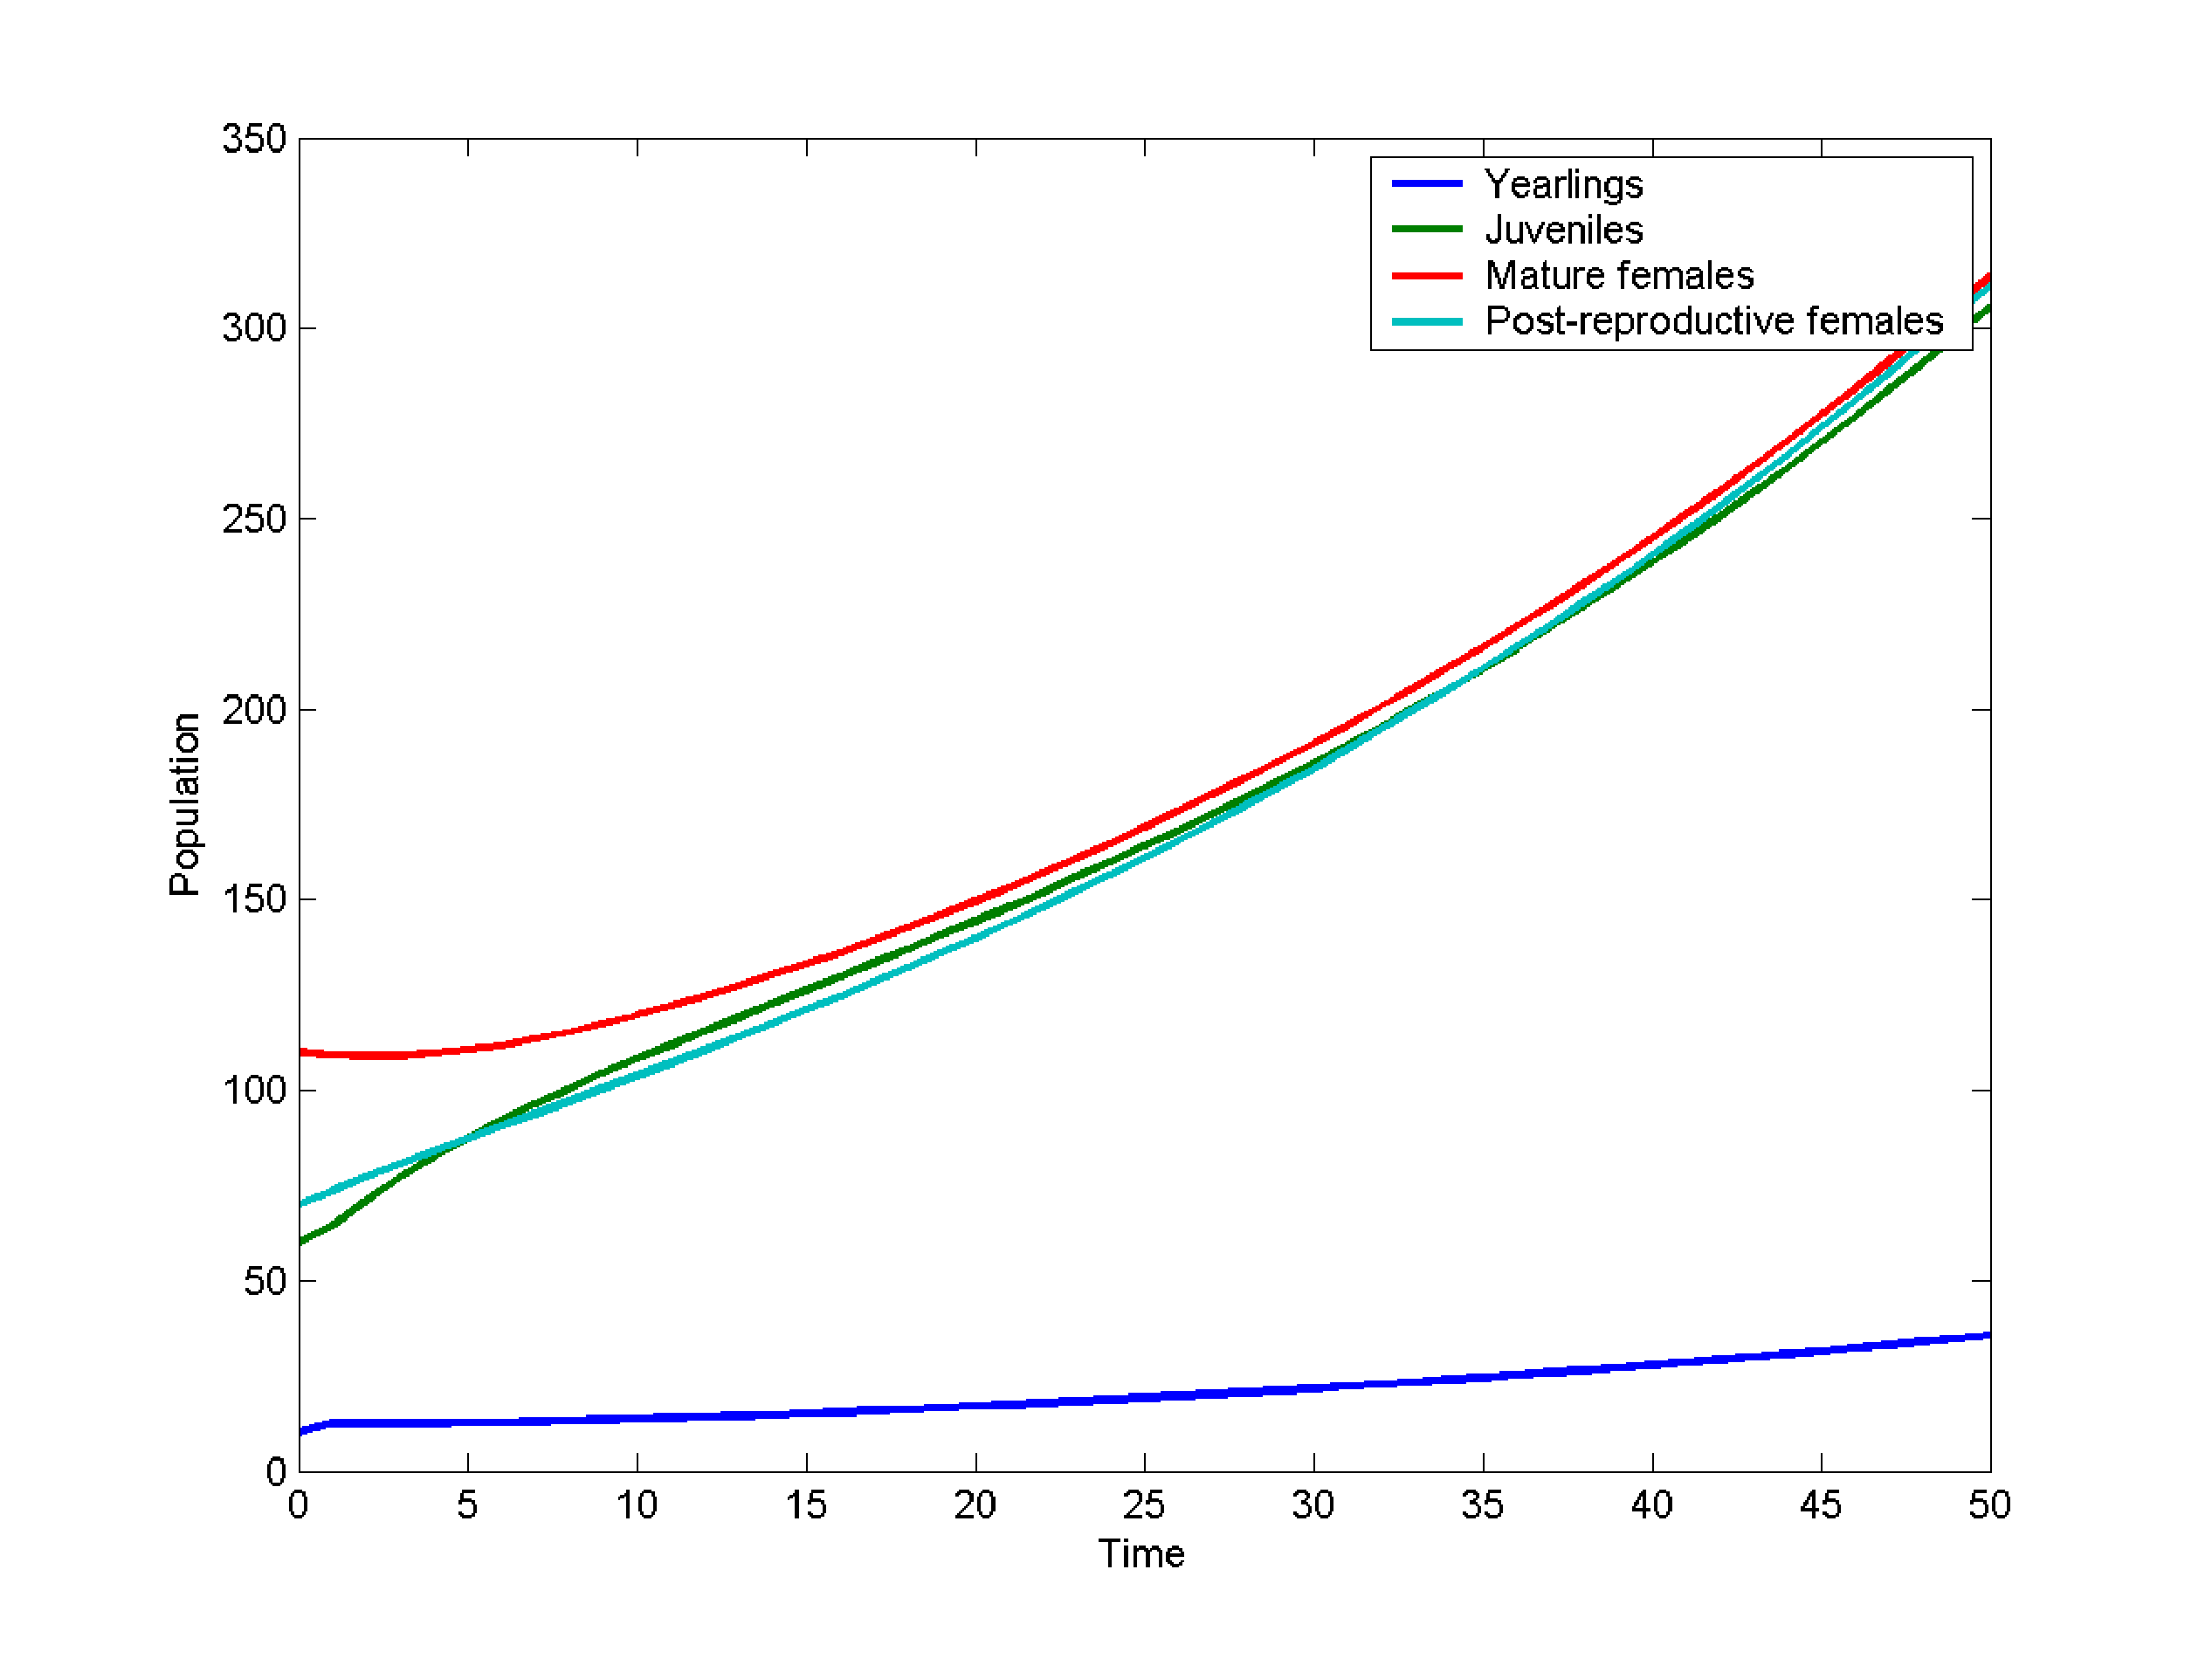
\includegraphics[width=.6\textwidth]{figs_steph/KillerWhales}
\end{center}


\subsubsection{Salmon population}
Suppose a population of salmon live to three years of age. Each adult salmon produces 800 offspring. The
probability of a salmon surviving the first year to live on to the second year is $5\%$, and the probability of a
salmon surviving the second year to live on to the third year is $2.5\%$.
\begin{itemize}
\item Find the Leslie matrix for this population.
\item If there are 10 females in each of the three age classes, find the initial age distribution vector. Use Matlab
to find the population age distribution vectors for each of the first 100 years.
\item Use Matlab to find the eigenvalues and eigenvectors of the Leslie Matrix. Is there a strictly dominant eigenvalue?
\item Describe what happens to this population of salmon over time?
\end{itemize}

\subsubsection{Human Population}
Suppose the population of the United States is broken up into ten 5-year age classes. The values for the
reproduction rates $F_i$ and the survival rates $P_i$ for each age class are shown in the table below.


\begin{tabular}{ccc}
i &$F_i$ & $P_i$\\
1 & 0 & 0.99670\\
2 &0.00102 &0.99837\\
3 &0.08515 &0.99780\\
4 &0.30574 &0.99672\\
5 &0.40002 &0.99607\\
6 &0.28061 &0.99472\\
7 &0.15260 &0.99240\\
8 &0.06420 &0.98867\\
9 &0.01483 &0.98274\\
10 &0.00089 &0
\end{tabular}
\begin{itemize}
\item Find the Leslie matrix for this population.
\item  If there are 10 females in each of the ten age classes, find the initial age distribution vector. Use Matlab to
find the population age distribution vectors for each of the first 100 years, and plot the age distribution
vectors.
\item  Use Matlab to find the eigenvalues and eigenvectors of the Leslie Matrix. What happens to this population
over time?
\item  After a long period of time, what is the relative number of females in each of the ten age classes?
%\item  After a long period of time, by what percentage is the population growing or shrinking?
\end{itemize}

\subsubsection{Insect population}
Insect Life cycle:
\begin{description}
\item[ADULT] 
The life cycle description can be started with the adult insect. The adult may be a beetle, fly, moth, or midge. Regardless of their form, insects mate and most lay eggs.
\item[EGG] 
Eggs come in many shapes, sizes, and colors. They might be deposited on or in the ground, the roots, the stems, the leaves, or the flowers. When the eggs hatch the new insect is called a larva. 
\item[LARVA]
The larva seldom looks like the adult it will become. Some common larval forms are the maggot, grub worm, inchworm, and caterpillar. As the larva grows it must shed it�s old skin from time to time. This is called molting. From hatching to the first molt the larva is said to be in it�s 1st instar stage. After molting the first time the larva enters it�s second instar stage, and so on. The feeding activity of the larvae often inflicts more damage on the noxious weed than the adult form. Different insects have different numbers of instars, but eventually the larva is fully grown and ready to pupate.
\item[PUPA] 
The pupa is the life stage between larva and adult. In this stage the insect does not feed, and can be considered motionless. This metamorphic change is often profound. Unless the larva is in a stem or root tunnel it will usually construct some kind of shelter to pupate in. This "cocoon" might be made from soil particles, silk, chewed seeds, chewed plant material, ground litter, or combinations.
Inside the "cocoon/shelter/chamber/capsule/case" the pupa is gradually transformed into an adult.
\end{description}
\begin{figure}
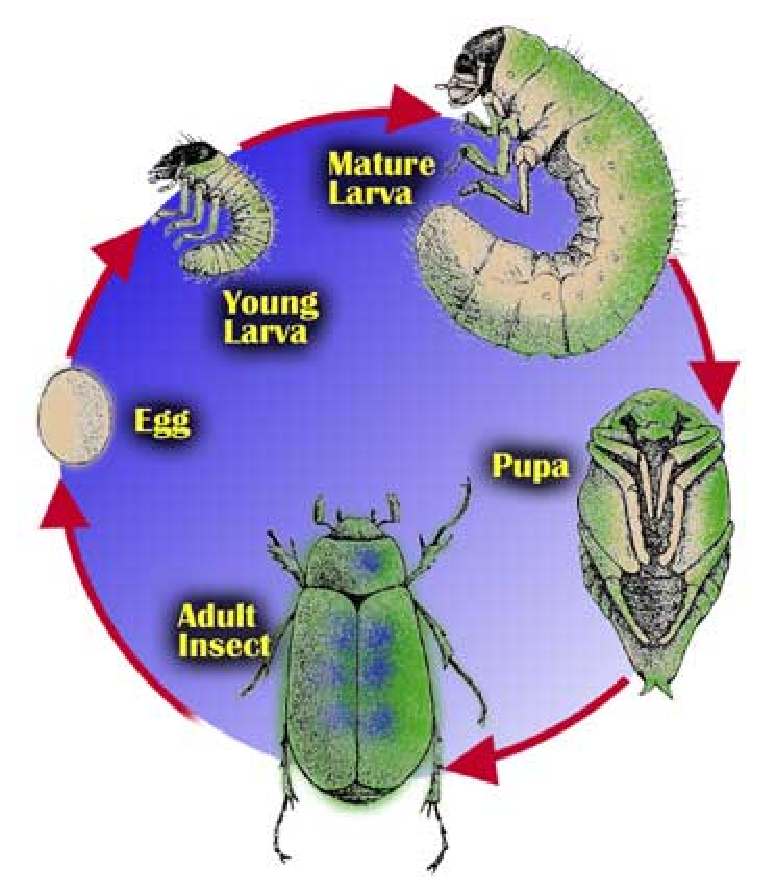
\includegraphics[width=.4\textwidth]{figs_steph/insect_life_cycle}
\caption{Example of insect life cycle}
\end{figure}

\subsection{Genetic model}
The simplest type of genetic inheritance of traits in animals occurs when a certain trait is determined by a specific pair of genes, each of which may be two types, say $G$ and $g$. An individual may have a $GG$ combination, a $Gg$ (genetically equivalent to $gG$), or $gg$ combination. An individual with $GG$ is said to be dominant, a $gg$ individual is recessive and a $Gg$ is an hybrid.

In the mating of two animals, the offspring inherits one gene of the pair from each parent: the basic assumption of genetics is that these genes are selected at
random, independently of each other.


This assumption determines the probability
of occurrence of each type of offspring: The offspring
\begin{itemize}
\item of two purely dominant parents
must be dominant, 
\item of two recessive parents must be recessive,
\item and of one dominant and one recessive parent must be hybrid.
\end{itemize}
In the mating of a dominant and a hybrid animal, each offspring must get a
G gene from the former and has an equal chance of getting G or g from the latter.
Hence there is an equal probability for getting a dominant or a hybrid offspring.
Again, in the mating of a recessive and a hybrid, there is an even chance for getting
either a recessive or a hybrid. In the mating of two hybrids, the offspring has an
equal chance of getting G or g from each parent. Hence the probabilities are 1/4
for GG, 1/2 for Gg, and 1/4 for gg.

Consider a process of continued matings. We start with an individual of known
genetic character and mate it with a hybrid. We assume that there is at least one
offspring. An offspring is chosen at random and is mated with a hybrid and this
process repeated through a number of generations. The genetic type of the chosen
offspring in successive generations can be represented by a Markov chain. The states
are dominant, hybrid, and recessive, and indicated by GG, Gg, and gg respectively:  3 possibles states $s_1=GG$, $s_2=Gg$ and $s_3=gg$.

Let $p_i(n)$ represent the probability that state $s_i$ occurs in the $n^{th}$ generation.
Let $p_{ij}$ be the probability that $s_i$ occurs in the $(n+1)^{th}$ generation given that $s_j$ occured in the $n^{th}$ generation.

The difference equation system that models the Markov chain is

$$
\begin{array}{ll}
p_1(n+1)=&p_{11}p_1(n)+p_{12}p_2(n)+p_{13}p_3(n)\\
p_2(n+1)=&p_{21}p_1(n)+p_{22}p_2(n)+p_{23}p_3(n)\\
p_3(n+1)=&p_{31}p_1(n)+p_{32}p_2(n)+p_{33}p_3(n)
\end{array}
$$


The transition probabilities are

$$S=\left (
\begin{array}{ccc}
0.5 & 0.25 & 0\\
0.5 & 0.5 & 0.5\\
0 & 0.25 & 0.5
\end{array}\right )
$$

$S$ is a stochastic matrix (nonnegative + sum of column equal to 1) $\Rightarrow$ $\rho(S)=1$


It is a regular Markov chain as $S^2>0$ (so $S$ is primitive).

Then the dominant eigenvalue $\lambda _1 =1$
and 

$$\lim_{n\rightarrow \infty }p(n)=cV_1$$
where $V_1=(0.41,0.82,0.41)^T$ is the eigenvector corresponding to $\lambda _1$, and is
$$c=\frac{1}{0.41+0.82+0.41}=0.609$$
Then
$$\lim_{n\rightarrow \infty }p(n)=\left ( 
\begin{array}{c}
0.25\\
0.5\\
0.25
\end{array}
\right )$$

As the number of repetitions approaches infinity, the probabilty of producing a purely dominant or purely recessive offspring is 0.25, and the probability of producing a hybrid offspring is $0.5$.




\section{Nonlinear difference equations}
Here, we study autonomous difference equations.

\subsection{Equilibrium solution - Periodic solution}
\begin{definition}\label{def:fixedpoint}
A point $x^*$ in the domain of $f$ is said to be an equilibrium point (an equilibrium solution) of the first-order difference equation $$x_{t+1}=f(x_t)$$ if it is a fixed point of $f$ \emph{i.e.} a constant solution that satisfies
$$f(x^*)=x^*.$$
\end{definition}
Graphically an equilibrium point is the $x-$coordinate of the point where the graph of $f(x)$ intersect the diagonal line $y=x$.


Same definition as in Definition \ref{def:fixedpoint} holds for a first-order system. For example, for a two-dimensional first order system
$$
\begin{array}{cc}
x_{t+1}=&f(x_t,y_t)\\
y_{t+1}=&g(x_t,y_t)
\end{array}
$$
the equilibrium solution is a solution $(\bar x, \bar y)$ such that $\bar x= f(\bar x,\bar y)$ and $\bar y=g(\bar x,\bar y)$.

\begin{quote}
Equilibrium solutions are biologically interesting because they represent the "resting states", the "stationary states" of the system. No change occurs from generation $t$ to generation $t+1$. 
\end{quote}



A difference equation takes the form
\[
x_{t+1}=f(x_t).
\]
Starting from an initial point $x_0$, we have
\begin{align*}
x_1 &= f(x_0) \\
x_2 &= f(x_1)=f(f(x_0))=f^2(x_0) \\
x_3 &= f(x_2)=f(f(f(x_0)))=f^3(x_0) \\
\ldots &\\
x_t &= f(f(f(\dots f(x_0))))=f^t(x_0)
\end{align*}
where the superscript $t$ is the number of time steps or iterations beginning from the initial value $x_0$. $f^m(x_0)$ is called the $m^{th}$ iterate of $f$.




\begin{definition}
A periodic solution of period $m>1$ of the difference equation $$x_{t+1}=f(x_t)$$ is a real-values solution $\bar x_k$ satisfying
$$f^m(\bar x_k)=\bar x_k$$ and $$f^i(\bar x_k)\not =\bar x_k \quad i=1,2,\dots, m-1$$
\end{definition}

\begin{quote}
Note that an equilibrium point is a solution of period 1.
\end{quote}


Graphically a periodic point is the $x-$coordinate of the point where the graph of $f^m(x)$ intersect the diagonal line $y=x$.
\vspace{.5cm}



\begin{definition}
An $m-$cycle is a set of points $\{\bar x _1, \bar x_2, \dots , \bar x_m\}$ where for each $k=1,\dots,m$, $\bar x_k$ is a periodic solution of period $m$. The set $\{\bar x_1, f(\bar x_1), \dots , f^{m-1}(\bar x_1) \}$ is called a periodic orbit of $\bar x_1$
\end{definition}



\subsection{Local stability in first-order equations}
Local stability of an equilibrium solution implies that solutions approach the equilibrium only if they are initially close to it. Global stability of an equilibrium is much stronger: global stability implies that regardless of the initial condition, solutions approach the equilibrium.

An equilibrium is called locally asymptotically stable if for any small perturbation away from the equilibrium, the solution returns to the equilibrium value.

\begin{definition}[Locally stable]
A equilibrium solution $\bar x$ of $x_{t+1}=f(x_t)$ is \emph{locally stable} if, for any  $\varepsilon>0$, there exists $\delta>0$ such that if $|x_0-\bar x|<\delta$, implies $$|x_t- \bar x|=|f^t(x_0)-\bar x|<\varepsilon \quad \forall t>0.$$ If a fixed point $\bar x$ is not stable, then it is \emph{unstable}.
\end{definition}


\begin{definition}[Locally attracting]
A equilibrium solution $\bar x$ is \emph{locally attracting} if there exists $\eta>0$ such that
\[
|x_0-\bar x|<\eta\quad\textrm{implies}\quad \lim_{t\to\infty}x_t=\bar x.
\]
If $\eta=\infty$, then $\bar x$ is a \emph{global attractor} (or is \emph{globally attracting}).
\end{definition}

\begin{definition}[Locally asymptotically stable]
The equilibrium solution $\bar x$ is locally asymptotically stable if it is locally stable and locally attracting.
\end{definition}

%Local asymptotic stability is referred to as \emph{neighborhood stability}. Solutions that are locally asymptotically stable converge to the stable equilibrium if they begin in a small neighborhood of that equilibrium.

The convergence behavoir for a first-order difference equation that is locally asymptotically stable may take the form of convergent oscillations or convergent exponential solutions. If the solution values tend to amplify and do note converge to the equilibrium,  the equilibrium is unstable. Such instability may appear as divergent oscillations or divergent exponential solutions. When the equilibrium is stable but not asymptotically stable it is said \emph{neutral stable}.


%To study local stability:
%\begin{itemize}
%\item identify the equilibrium solution
%\item linearization techniques to determine the behavior of solution near the equilibrium.
%\item If the equilibrium is stable for any set of initial condition, then the equilibrium is globally stable.
%\end{itemize}

\vspace{1cm}
Let define a difference equation
\begin{equation}\label{eq:NonLin}
x_{t+1}=f(x_t)
\end{equation}
with an equilibrium solution $\bar x$. Let define a new variable
$$u_{t}=x_t-\bar x.$$
$u_t$ is a small quantity termed a perturbation of the equilibrium solution. Then $u_t$ satisfies the difference equation \eqref{eq:NonLin}
$$u_{t+1}=x_{t+1}-\bar x=f(x_t)-\bar x=f(u_t+\bar x)-f(\bar x)=g(u_t)$$
where $g(u)=f(u+\bar x)-f(\bar x)$.

Note that zero is a fixed point of $g$ if and only if $\bar x$ is a fixed point of $f$. In addition, zero is a locally stable (unstable, or locally asymptically stable) fixed point of $g$ if and only if $\bar x$ is a locally stable (unstable or locally asymptotically stable) fixed point of $f$. To find for the stability of $\bar x$ we assume that $f$ has a second order derivative in some interval $I$ containing $\bar x$, then by Taylor's approximation
$$f(x)=f(\bar x)+f'(\bar x)(x-\bar x)+\frac{f''(\epsilon)}{2!}(x-\bar x)^2$$
for $\epsilon \in I$. For $(x-\bar x)$ sufficiently small, we have the linear approximation
$$\underbrace{f(x_t)-\bar x}_{u_{t+1}}=f'(\bar x)\underbrace{(x_t-\bar x)}_{u_t},$$
then 
\begin{equation}\label{eq:Linearizatio}
u_{t+1}=f'(\bar x)u_t
\end{equation} is referred to as the \emph{linear approximation} to the difference equation \eqref{eq:NonLin} at the equilibrium $\bar x$.

If the initial condition are sufficiently close to $\bar x$, then the dynamics of $u_t$ is determined by the linearization \eqref{eq:Linearizatio}. In term of perturbation, to understand whether small perturbations $u_t$ from the equilibrium solution increase or decrease, we can solve \eqref{eq:Linearizatio} by using the difference equation method. We know that the solution of \eqref{eq:Linearizatio} will be decreasing whenever $|f'(\bar x)|<1$. Therefore, the value of $f'(\bar x)$ determines whether $\bar x$ is locally asymptotically stable or unstable.



\begin{theorem}[Condition for stability]
Assume  $f'$ is continuous on an open interval $I$ containing $\bar x$ and $\bar x$ is a fixed point of $f$. Then $\bar x$ is a locally asymptotically stable equilibrium of $x_{t+1}=f(x_t)$ if
$$|f'(\bar x)|<1$$
and unstable if $$|f'(\bar x)|>1$$
\end{theorem}




\begin{definition}
An equilibrium $\bar x$ of $$x_{t+1}=f(x_t)$$ is said to be hyperbolic if $|f'(\bar x)|\not =1$.

Otherwise ($|f'(\bar x)| =1$), it is said to be nonhyperbolic.
\end{definition}

\begin{theorem}
Suppose that $f'(\bar x) =1$ for an equilibrium solution $\bar x$ of $x_{t+1}=f(x_t)$, and $f'''$ is continuous on an open interval containing $\bar x$, then the following statement hold:
\begin{itemize}
\item $f''(\bar x)\not =0$, then the $\bar x$ is unstable.
\item $f''(\bar x)=0$ and $f'''(\bar x)>0$, then $\bar x$ is unstable.
\item $f''(\bar x)=0$ and $f'''(\bar x)<0$, then $\bar x$ is locally asymptotically stable.
\end{itemize}
\end{theorem}

\begin{definition}[Schwarzian derivative]
The Schwarzian derivative of a function $f$ at $x$ is denoted $(Sf)(x)$ and defined as follows:
$$(Sf)(x)=\frac{f'''(x)}{f'(x)}-\frac{3}{2}\left ( \frac{f''(x)}{f'(x)} \right )^2.$$
\end{definition}
Note that $f'(x)=-1$, $(Sf)(x)=-f'''(x)-\frac{3}{2} f''(x)^2.$
\begin{theorem}
Suppose that $f'(\bar x) =-1$ for an equilibrium solution $\bar x$ of $x_{t+1}=f(x_t)$, and $f'''$ is continuous on an open interval containing $\bar x$, then the following statement hold:
\begin{itemize}
\item $(Sf)(\bar x)>0$, then the $\bar x$ is unstable.
\item $(Sf)(\bar x)<0$, then $\bar x$ is locally asymptotically stable.
\end{itemize}
\end{theorem}




\begin{theorem}
Suppose $f'$ is continuous on an open interval $I$ and the $m-$cycle
$$\{\bar x_1, f(\bar x_1), \dots , f^{m-1}(\bar x_1)\}$$
of the difference equation $$x_{t+1}=f(x_t)$$ is contained in $I$. Then the $m-$cycle is locally asympotically stable if
$$\left| \frac{d[f^m(\bar x_k)]}{dx}\right|<1$$
for some $k$ and unstable if
$$\left| \frac{d[f^m(\bar x_k)]}{dx}\right|>1$$
for some $k$.
\end{theorem}



\begin{theorem}(Corollary)
Suppose $\{\bar x_1, \bar x_2, \dots , \bar x_m\}$ is an $m-$cycle of $x_{t+1}=f(x_t)$. Then the $m-$cycle is locally asymptotically stable if $$\left |   f'(\bar x_1)f'(\bar x_2)\dots f'(\bar x_m)\right |<1$$
\end{theorem}


Illustration: $\{\bar x_1,\bar x_2\}$ is a $2-$cycle that is locally asymptotically stable if and only if $$\left| \left . \frac{d[f]}{dx}\right |_{\bar x_1}\left . \frac{d[f]}{dx}\right |_{\bar x_2}\right|<1$$


\subsubsection{Cobwebbing method for first-order equation}
Graphical method to answer qualitative questions about the solution of $$x_{t+1}=f(x_t).$$

In the $(x_tx_{t+1})-$plane, sketch $x_{t+1}=x_{t}$ and $x_{t+1}=f(x_t)$:
\begin{itemize}
\item any intersections of these graphs is an equilibrium solution of the difference equation.
\item to investigate the behavior of the solutions
\begin{itemize}
\item choose a starting value $x_0$, and begin at the point $(x_0,x_0)$ in the $(x_tx_{t+1})-$plane.
\item draw a vertical line to the curve $x_{t+1}=f(x_t)$; this reaches the curve at $(x_0,f(x_0))=(x_0,x_1)$.
\item draw a horizontal line to the diagonal $x_{t+1}=x_t$; this reaches the diagonal at the point $(x_1,x_1)$.
\item Repeat the process to arrive at $(x_2,x_2)$ and indefinitely until the behavior of the equation with this starting value becomes clear.
\item If necessary, re-do the same with other starting values.
\end{itemize}
\end{itemize}




\subsection{Global stability in first-order equations}
Global stablity of an equilibrium removes the restrictions on the initial conditions. In global asympotic stability, solutions approach the equilibrium solution for all initial conditions. 


\begin{definition}
Suppose that $\bar x$ is an equilibrium solution of the difference equation $$x_{t+1}=f(x_t),$$
where $f: [0,a)\rightarrow [0,a),$ $0<a\leq \infty$. Then $\bar x$ is said to be globally attractive if for all initial conditions $x_0\in (0,a)$, $$\lim_{t\rightarrow \infty}x_t=\bar x.$$

The equilibrium is said to be globally asymptotically stable if $\bar x$ is globally attractive and if $\bar x$ is locally stable.
\end{definition}
Globally attractive equilibria are locally attractive, therefore globally asymptotically stable equilibria are locally asymptotically stable.


If $f$ is a continuous map, global attractivity is equivalent to global asymptotic stability.


\begin{theorem}
If the fucntion $f$ of $x_{t+1}=f(x_t)$ satisfies
\begin{itemize}
\item $f$ is continuous on $[0,a),$ $0<a\leq \infty$,
\item $f: [0,a)\rightarrow [0,a),$ $0<a\leq \infty$,
\item $0<f(x)<x$ for all $x\in [0,a)$,
\end{itemize}
 then the origin is globally asymptotically stable.
\end{theorem}

Necessary and sufficient conditions for global asymptotic stability of a positive equilibrium $\bar x$

\begin{theorem}
The difference equation $x_{t+1}=f(x_t)$ satisfying 
\begin{itemize}
\item $f$ is continuous on $[0,a),$ $0<a\leq \infty$,
\item $f: [0,a)\rightarrow [0,a),$ $0<a\leq \infty$,
\item $f(0)=0$, $f(\bar x)=\bar x$ 
\item $f(x)>x$ for $0<x<\bar x$
\item $f(x)<x$ for $\bar x<x<a$
\item if $f$ has a maximum at $x_M$ in $(0,\bar x)$, then $f$ is decreasing for $x>x_M$
\end{itemize}
has a globally asymptotically stable equilibrium at $\bar x$ if and only if $f$ has no 2-cycles.
\end{theorem}

\begin{theorem}
Let $f'$ be continuous on an interval $I$ and $f: I\rightarrow I$. If $1+f'(x)\not =0$ for all $x\in I$ then $x_{t+1}=f(x_t)$ has no $2-cycles$ in $I$.
\end{theorem}

\begin{theorem}
If $f$ satisfies
\begin{itemize}
\item $f$ is continuous on $[0,a),$ $0<a\leq \infty$,
\item $f: [0,a)\rightarrow [0,a),$ $0<a\leq \infty$,
\item $\bar x \in (0,a)$ such that $x<f(x)<\bar x$ for $0<x<\bar x$
and $\bar x<f(x)< x$ for $x>\bar x$
\end{itemize}
then the difference equation $x_{t+1}=f(x_t)$ has a globally asymptotically stable equilibrium at $\bar x$.
\end{theorem}

\begin{theorem}\label{theo:2.9}
Let $x_{t+1}=f(x_t)$
\begin{description}
\item[a) ]Suppose that $f$ satisfies
\begin{itemize}
\item $f$ is continuous on $[0,a),$ $0<a\leq \infty$,
\item $f: [0,a)\rightarrow [0,a),$ $0<a\leq \infty$,
\item $f(0)=0$, $f(\bar x)=\bar x$ 
\item $f(x)>x$ for $0<x<\bar x$
\item $f(x)<x$ for $\bar x<x<a$
\end{itemize}
but has no maximun in $(0,\bar x)$. Then $\bar x$ is globally asymptotically stable.
\item[b) ]Suppose that $f$ satisfies
\begin{itemize}
\item $f$ is continuous on $[0,a),$ $0<a\leq \infty$,
\item $f: [0,a)\rightarrow [0,a),$ $0<a\leq \infty$,
\item $f(0)=0$, $f(\bar x)=\bar x$ 
\item $f(x)>x$ for $0<x<\bar x$
\item $f(x)<x$ for $\bar x<x<a$
\item if $f$ has a maximum at $x_M$ in $(0,\bar x)$, then $f$ is decreasing for $x>x_M$
\end{itemize}
has a maximun $x_M$ in $(0,\bar x)$. Then $\bar x$ is globally asymptotically stable if and only if $f(f(x))>x$ for all $x\in [x_M,\bar x)$
\end{description}
\end{theorem}


\subsection{Bifurcation diagrams}
To summarize the range of behaviors, a diagram of bifurcation can be used by  depicting the locations and the stability properties of periodic solutions. To illustrate the effect of a parameter variation on existence and stability properties of periodic solutions. 

Dependence of a difference equation on a parameter can be noted
$$x_{t+1}=f(x_t,r).$$
The values of $r$ where the behavior changes are known as the \emph{bifurcation values} and the points $(r,\bar x(r))$ are the \emph{bifurcation points}  with $\bar x(r)$ is the value of periodic solutions for the parameter value $r$.

A change in the solution behavior occurs when an equilibrium or a $m-$cycle changes stability.

\begin{itemize}
\item on the horizontal axis, the parameter value $r$.
\item on the vertical axis, the magnitudes of equilibrium solutions or cycles.
\item an unstable equilibrium or cycle is denoted by a dashed curve.
\item a stable equilibrium or cycle is denoted by a solid curve.
\end{itemize}


\begin{definition}
Deterministic chaos is a pattern of fluctuations that may seem to be stochastic but it is actually produced in a deterministic manner, by autonomous nonlinear dynamic processes.
\end{definition}

A property of the chaotic system is the extrem sensitivity to initial conditions. 
\begin{quote} 
Sensitive dependence to initial conditions means that
a small perturbation in these initial conditions will grow exponentially with time. Even
if, theoretically, it should be possible to predict the future dynamic as a function of
time, in reality it is impossible, because the smallest error in the specification of the
initial state leads to a great error in future predictions. In fact, in deterministic chaos,
the knowledge of the state of the system during as long a time as we want, doesn't
allow us to predict its further evolution \cite{Glass1988}.
\end{quote}

A chaotic system has cycles of every period.

\subsection{Systems of nonlinear equations}
Consider the system
\begin{equation}
\begin{array}{cc}
x_{t+1}=& f(x_t,y_t)\\
y_{t+1}=& g(x_t,y_t)
\end{array}\label{eq:SysNonlinear2}
\end{equation}
where $f$ and $g$ are nonlinear function. The equilibrium $(\bar x, \bar y)$ satisfies
$$\bar x=f(\bar x,\bar y),$$
$$\bar y=g(\bar x,\bar y).$$

What is the stability of the equilibrium $(\bar x, \bar y)$?

First step: linearization of the system about the equilibrium.


To linearize the system, we use Taylor series expansions of functions of two varibale to approximate $f$ and $g$ about $(\bar x, \bar y)$.
$$f(x,y)= f(\bar x,\bar y)+\left .\frac{\partial f}{\partial x}\right |_{\bar x,\bar y}(x-\bar x)+ \left .\frac{\partial f}{\partial y}\right |_{\bar x,\bar y}(y-\bar y)+ \left .\frac{\partial^2 f}{\partial x^2}\right |_{\bar x,\bar y}\frac{(x-\bar x)^2}{2!} + \left .\frac{\partial^2 f}{\partial y^2}\right |_{\bar x,\bar y}\frac{(y-\bar y)^2}{2!} \dots $$

$$f(x,y)= f(\bar x,\bar y)+\left .\frac{\partial f}{\partial x}\right |_{\bar x,\bar y}(x-\bar x)+ \left .\frac{\partial f}{\partial y}\right |_{\bar x,\bar y}(y-\bar y)$$
Consider a small perturbations $u=x-\bar x$ and $v=y-\bar y$, then 
$$f(x,y)= f(\bar x,\bar y)+\left .\frac{\partial f}{\partial x}\right |_{\bar x,\bar y}u+ \left .\frac{\partial f}{\partial y}\right |_{\bar x,\bar y}v$$
and 
$$g(x,y)= g(\bar x,\bar y)+\left .\frac{\partial g}{\partial x}\right |_{\bar x,\bar y}u+ \left .\frac{\partial g}{\partial y}\right |_{\bar x,\bar y}v$$
Then,
$$f(x,y)- \bar x=\left .\frac{\partial f}{\partial x}\right |_{\bar x,\bar y}u+ \left .\frac{\partial f}{\partial y}\right |_{\bar x,\bar y}v$$
$$g(x,y)-\bar y=\left .\frac{\partial g}{\partial x}\right |_{\bar x,\bar y}u+ \left .\frac{\partial g}{\partial y}\right |_{\bar x,\bar y}v$$
As $u_t=x_t-\bar x$, $v_t=y_t-\bar y$ and $u_{t+1}=x_{t+1}-\bar x$, $v_{t+1}=y_{t+1}-\bar y$ then $u_{t+1}=f(x_t,y_t)-\bar x$, $v_{t+1}=g(x_t, y_t)-\bar y$. Therefore
$$u_{t+1}=f(x_t,y_t)- \bar x=\left .\frac{\partial f}{\partial x}\right |_{\bar x,\bar y}u_t+ \left .\frac{\partial f}{\partial y}\right |_{\bar x,\bar y}v_t$$
$$v_{t+1}=g( x_t, y_t)-\bar y=\left .\frac{\partial g}{\partial x}\right |_{\bar x,\bar y}u_t+ \left .\frac{\partial g}{\partial y}\right |_{\bar x,\bar y}v_t$$

The linearization of \eqref{eq:SysNonlinear2} about the equilibrium $(\bar x, \bar y)$ where $u_t=x_t-\bar x$ and  $v_t=y_t-\bar y$ is

$$V_{t+1}=JV_t$$
where $V_{t}=(u_t,v_t)^T$ and $J$ is the Jacobian of $(f,g)^T$ evaluated at $(\bar x, \bar y)$
$$
J=\left ( 
\begin{array}{cc}
\left . \frac{\partial f}{\partial x}\right |_{\bar x,\bar y} & \left .\frac{\partial f}{\partial y}\right |_{\bar x,\bar y}\\
\left .\frac{\partial g}{\partial x}\right |_{\bar x,\bar y} & \left .\frac{\partial g}{\partial y}\right |_{\bar x,\bar y}\\
\end{array}
\right )
=
\left ( 
\begin{array}{cc}
a_{11} & a_{12} \\
a_{21} & a_{22}
\end{array}
\right )
$$
The eigenvalues of the Jacobian $J$ determine the local stability of the nonlinear system. If the eigenvalues satifies $|\lambda _i|<1$ so that the spectral radius $\rho (J)<1$, then from Theorem \ref{Theorem:MatrixConverg} $\lim _{t\rightarrow \infty} J^t=0$.



To find the eigenvalues of $J$ we need to solve 
$$\det (J-\lambda I)=\det \left ( 
\begin{array}{cc}
a_{11}-\lambda & a_{12} \\
a_{21} & a_{22} -\lambda
\end{array}
\right )=0.$$
The characteristic equation is
$$\lambda ^2 -(a_{11}+a_{22})\lambda + a_{11}a_{22}-a{12}a_{21}=\lambda ^2 -\tr(J)\lambda + \det (J)=0$$
then the eigenvalues are
$$\lambda_{1,2}=\frac{\tr(J)\pm \sqrt{\tr(J)^2-4\det (J)}}{2}$$

\begin{theorem}\label{theo:stable2dim}
Let $f(x,y)$ and $g(x,y)$ be two functions with continuous first-order partial derivatives in $x$ and $y$ on some set containing $(\bar x, \bar y)$. Then the equilibrium $(\bar x, \bar y)$ of the nonlinear system
$$
\begin{array}{cc}
x_{t+1}=& f(x_t,y_t)\\
y_{t+1}=& g(x_t,y_t)
\end{array}$$
is locally asymptotically stable if the eigenvalues of the Jacobian matrix $J$ evaluated at  the equilibrium $(\bar x, \bar y)$ satisfy $|\lambda _i|<1$ if and only if
$$|\tr(J)|<1+\det (J)<2.$$

The equilibrium is unstable if some $|\lambda _i|>1$, that is, if any one of three inequalities is satisfied
\begin{itemize}
\item $\tr(J)>1 + \det (J),$
\item or $\tr(J)<-1 - \det (J),$
\item or $\det (J)>1$
\end{itemize}
\end{theorem}

See Figure \ref{fig:THeoStable} for illustration

\begin{figure}\label{fig:THeoStable}
\includegraphics[width=.8\textwidth]{Eigen}
\caption{The triangular region inside the dashed lines is the region of local asymptotic stability $|\lambda _i|<1$ for the system of difference equations in the $\tr(J)-\det (J)-$plane. The solid curve represents $\tr(J)^2=4\det (J)$, below the curve the eigenvalues are real and above it the eigenvalues are complex. If the parameters lie outside of the triangular region tehn at least one eigenvalue satisfies $|\lambda _i|>1$.}
\end{figure}


\subsubsection{Higher-order difference equations}
Local stability criteria for first or higher order difference equation depend on the behavior of the linearization of the system.

Consider a first-order system of $n$ nonlinear equations $X(t)=(x_1(t),x_2(t), x_3(t), \dots , x_n(t))^T$
$$X(t+1)=F(X(t))$$
where $F=(f_1,f_2,f_3, \dots , f_n)^T$ with $f_i=f_i(x_1,x_2,x_3,\dots , x_n)$ for $i=1,2,3,\dots ,n$. The point $\bar X$ is an equilibrium of the $n-$dimensional nonlinear system.

If $U(t)=X(t)-\bar X$, the linearization of the $n-$dimensional nonlinear system about $\bar X $ is
$$U(t)=J U(t)$$
where $J$ is the Jacobian matrix evaluated at $\bar X$
$$
J=\left ( 
\begin{array}{cccc}
\frac{\partial f_1 (\bar X)}{\partial x_1} & \frac{\partial f_1 (\bar X)}{\partial x_2} & \hdots & \frac{\partial f_1 (\bar X)}{\partial x_n}\\
\frac{\partial f_2 (\bar X)}{\partial x_1} & \frac{\partial f_2 (\bar X)}{\partial x_2} & \hdots & \frac{\partial f_2 (\bar X)}{\partial x_n}\\
\vdots & \vdots & \hdots & \vdots \\
\frac{\partial f_n (\bar X)}{\partial x_1} & \frac{\partial f_n (\bar X)}{\partial x_2} & \hdots & \frac{\partial f_n (\bar X)}{\partial x_n}
\end{array}
\right )
$$ 
The eigenvalues of the Jacobian $J$ determine the local stability of the $n-$dimensional nonlinear system. Eigenvalues are solutions of the characteristic equation
$$\det (J -\lambda I)=0.$$
The eigenvalues $\lambda $ are the zeros of the following $n^{th}$degree characteristic equation
\begin{equation}
p(\lambda)=\lambda ^n + a_1 \lambda ^{n-1}+ a_2 \lambda ^{n-2}+a_3 \lambda ^{n-3}+\dots + a_n\label{eq:CharacN}
\end{equation}
The conditions that must be satisfied for local asymptotic stability are known as the Jury Conditions or Schur-Cohn Criteria: they ensure that $|\lambda _i|<1$.

\begin{theorem}[Jury conditions or Schur-Cohn Criteria, for $n=3$]
Consider the characteristic polynomial $$p(\lambda)=\lambda ^n + a_1 \lambda ^{n-1}+ a_2 \lambda ^{n-2}+a_3 .$$
The solutions $\lambda _i$, $i=1,2,3,$ of $p(\lambda)=0$ satisfy $|\lambda _i|<1$ if and only if the following three conditions hold:
\begin{enumerate}
\item $p(1)=1+a_1+a_2+a_3>0,$
\item $(-1)^3p(-1)=1-a_1+a_2-a_3>0$
\item $1-(a_3)^2>|a_2 -a_3a_1|$
\end{enumerate}
\end{theorem}


Some necessary conditions for $|\lambda _i|<1$:
\begin{theorem}
If the solutions $\lambda _i$, $i=1,2,\dots , n$ of $$p(\lambda)=\lambda ^n + a_1 \lambda ^{n-1}+ a_2 \lambda ^{n-2}+a_3 \lambda ^{n-3}+\dots + a_n=0$$
satisfy $|\lambda _i|<1$ then
\begin{itemize}
\item $p(1)>0$
\item $(-1)^np(-1)>0$
\item $|a_n|<1$
\end{itemize}
\end{theorem}



%More dimensions... (just to know that these exist... but don't bother...)
%\begin{definition}
%The inners of a matrix $B=b_{i,j}$ are the matrix itself and all the matrices obtained by omitting successively the first and last rows and the first and last columns.
%\end{definition}
%
%\begin{theorem}[Jury conditions or Schur-Cohn Criteria]
%Consider the characteristic polynomial $$p(\lambda)=\lambda ^n + a_1 \lambda ^{n-1}+ a_2 \lambda ^{n-2}+a_3 \lambda ^{n-3}+\dots + a_n,$$
%with real coefficients. Define two $(n-1)\times(n-1)$ matrices $B_{n-1}^{\pm}$
%$$B_{n-1}^{\pm}=\left ( 
%\begin{array}{ccccc}
%1 & a_1 & a_2 & \hdots & a_{n-1} \\
%0 & 1   & a_2 & \hdots & a_{n-2} \\
%0 & 0   & 1   & \ddots & a_{n-3} \\
%\vdots & \vdots  & \vdots   & \ddots & \vdots \\
%0 & 0   & 0   & \hdots & 1
%\end{array}
%\right )
%\pm
%\left ( 
%\begin{array}{ccccc}
%0 & 0 & 0 & \hdots & a_{n} \\
%\vdots & \vdots   & \vdots & \hdots & \vdots \\
%0 & 0   & a_n & \hdots & a_{4} \\
%0 & a_n   &  a_{n-1}  & \ddots & a_3 \\
%a_n & a_{n-1}   & a_{n-2}   & \hdots & a_2
%\end{array}
%\right )
%$$
%The solution $\lambda _i$, $i=1,2,3, \dots ,n$ of $p(\lambda)=0$ satisfy $|\lambda _i|<1$ if and only if the following three conditions hold:
%\begin{enumerate}
%\item $p(1)>0,$
%\item $(-1)^np(-1)>0$
%\item the determinant of each of the inner matrices of $B_{n-1}^{\pm}$ are positive.
%\end{enumerate}
%\end{theorem}



\section{Examples}
\subsection{Single species models}
The population dynamics of single species with seasonal
reproduction and first-order feedback are often modelled
using a single difference equation.

\subsubsection{Discrete logistic model}
The logistic model (in differential equation formalism) is
$$\frac{dN}{dt}=a(1-\frac{N}{K})N$$
where $a$ is the intrinsic rate of growth of the population $N$ and $K$ represents the carrying capacity of the environment (the maximal number of individuals that the environment can support). For $N(0)>0$, $\lim _{t\rightarrow + \infty} N(t)=K$.

To derive the discrete logistic equation:
$$\frac{dN}{dt}=\frac{N(t+1)-N(t)}{\Delta t}$$
as previuously $\Delta t=1$ then
$$N(t+1)-N(t)=a(1-\frac{N(t)}{K})N(t)$$
$$N(t+1)=(a+1)N(t)-\frac{aN(t)^2}{K}$$
To study the discrete logistic model, we adimensionalize the model by using the change of variable $x_t=\frac{a}{K(1+a)}N(t)$ to obtain
$$x_{t+1}=(1+a)x_t(1-x_t)$$
and $1+a=\mu$.


{\bf Study of the adimensionless logistic model:} 
We consider the logistic growth function
\begin{equation}\label{eq:logistic_map}
f_\mu(x)=\mu x(1-x),
\end{equation}
used to define the discrete time logistic equation
\begin{equation}
x_{t+1}=f_\mu(x_t), \label{eq:logistic}
\end{equation}
the latter being considered with initial condition $x_0\in[0,1]$. It is assumed throughout that $0<\mu<4$.

{\bf Fixed points: }
ixed points of \eqref{eq:logistic_map} are found by solving the fixed point equation
\[
f_\mu(x)=x,
\]
that is,
\[
\mu x(1-x)=x.
\]
It is clear that there are two points that satisfy this equation, namely $x=0$ and $x=(\mu-1)/\mu$. We denote from now on $p=(\mu-1)/\mu$.

Remember that we are modelling a population, so we want $p>0$ (or at least, nonnegative). If $p>0$, we say that $p$ is \emph{biologically relevant}. For this, we need $\mu>1$. In the case that $\mu<1$, then $p$ does exist, but we do not consider it, as it is not biologically relevant, and by abuse of language, say that $p$ does not exist.

The fixed point $x=0$ always exists, and
\begin{itemize}
\item if $\mu\in(0,1)$, then $p$ does not exist,
\item if $\mu>1$, then $p$ exists.
\end{itemize}


{\bf Stability of fixed points: }
The derivative of the logistic growth function is
\begin{equation}\label{eq:dlogistic_map}
f_\mu'(x)=\mu-2\mu x=\mu(1-2x).
\end{equation}
To determine the stability of a fixed point $x^*$, we need to compare $|f'_\mu(x^*)|$ with the value 1. From \eqref{eq:dlogistic_map},
\[
|f_\mu'(0)|=|\mu|=\mu,
\]
and
\begin{align*}
|f_\mu'(p)| &= \left|\mu\left(1-2\frac{\mu-1}{\mu}\right)\right| \\
&= |1-2\mu|.
\end{align*}
As a consequence, $x=0$ is locally asymptotically stable if $\mu<1$ and unstable otherwise, and $p=(\mu-1)/\mu$ is locally asymptotically stable if $1-2\mu<1$, that is, $\mu<3$, and unstable otherwise.

\vskip0.5cm
\noindent Therefore
\begin{itemize}
\item if $\mu\in(0,1)$, then $x=0$ is locally asymptotically stable, and the fixed point $x=p$ does not exist,
\item if $\mu\in(1,3)$, then $x=0$ is unstable, and the fixed point $x=p$ exists and is locally asymptotically stable,
\item if $\mu>3$, then $x=0$ is unstable, and the fixed point $x=p$ exists and is unstable.
\end{itemize}


{\bf $2-$cycle: }
We now study the existence of periodic points period 2, that is, fixed points of $f_\mu^2(x)$:
\begin{align}
f_\mu^2(x) &= f_\mu(f_\mu(x)) =x \nonumber\\
& \mu^2 x(1-x)(1-\mu x(1-x))=x. \label{eq:f_mu_2_a}
\end{align}
Simplifying, we obtain
$$x(\mu x -(\mu -1))(\mu ^2x^2-\mu (\mu +1)x+\mu +1)=0.$$
Remark that 0 and $p$ are points of period 1. Indeed, a fixed point $x^*$ of $f$ satisfies $f(x^*)=x^*$, and as a consequence, $f^2(x^*)=f(f(x^*))=f(x^*)=x^*$. The points of period 2, constituting the $2-$cycle are:
$$\bar x_{1,2}=\frac{\mu +1\pm\sqrt{(\mu+1)^2-4(\mu+1)}}{2\mu}=\frac{\mu +1\pm\sqrt{(\mu -3)(\mu +1)}}{2\mu}$$
The $2-$cycle exists if $\mu >3$.


{\bf Stability of the $2-$cycle: }
The $2-$cycle is locally asymptotically stable is 

$|f_{\mu}'(\bar x_1)f_{\mu}'(\bar x_2)|<1$.

From \eqref{eq:dlogistic_map}, we obtain
$$|\left ( \mu -(\mu +1)+\sqrt{(\mu -3)(\mu +1)} \right )\left ( \mu-(\mu +1)-\sqrt{(\mu -3)(\mu +1)} \right )|<1$$
or $$|1-(\mu -3)(\mu +1)|<1$$
$$0<(\mu -3)(\mu +1)<2$$
Then $0<\mu ^2 -2\mu -3<2$, these inequalities are satisfied if 
$$3<\mu < 1+\sqrt{6}.$$
The $2-$cycle is unstable if $\mu > 1 +\sqrt{6}$.

{\bf Global stability}
By theorem \ref{theo:2.9} the equilibrium $p$ is globally asymptotically stable for $1<\mu<3$.

{\bf Bifurcation}
At $\mu =1$, $\mu =3$ and $\mu =1 + \sqrt{6}$ there are changes in stability of equilibria. Then $\mu =1$, $\mu =3$ and $\mu =1 + \sqrt{6}$ are bifurcation values. At $\mu =1$, the bifurcation is called a transcritical bifurcation. At $\mu =3$ and $\mu =1 + \sqrt{6}$, the bifurcation is called a period-doubling bifurcation. 

The analysis of the logistic growth can be continued to find bifurcation values:
\begin{itemize}
\item $\mu = 3.5441$ : for $1 + \sqrt{6}<\mu <3.5441$ there is a stable $4-$cycle
\item $\mu = 3.5644$ : for the parameter $3.5441<\mu <3.5644$ there is a stable $8-$cycle
\item $\mu = 3.5688$ : for the parameter $3.5644<\mu <3.5688$ there is a stable $16-$cycle
\item ... other stable cycle of increasing period $2^n$
\item $\mu > 3.57$ a cycle of period $3$ exits what is referred as chaotic solutions.
\end{itemize}
\begin{figure}[htbp]
\begin{center}
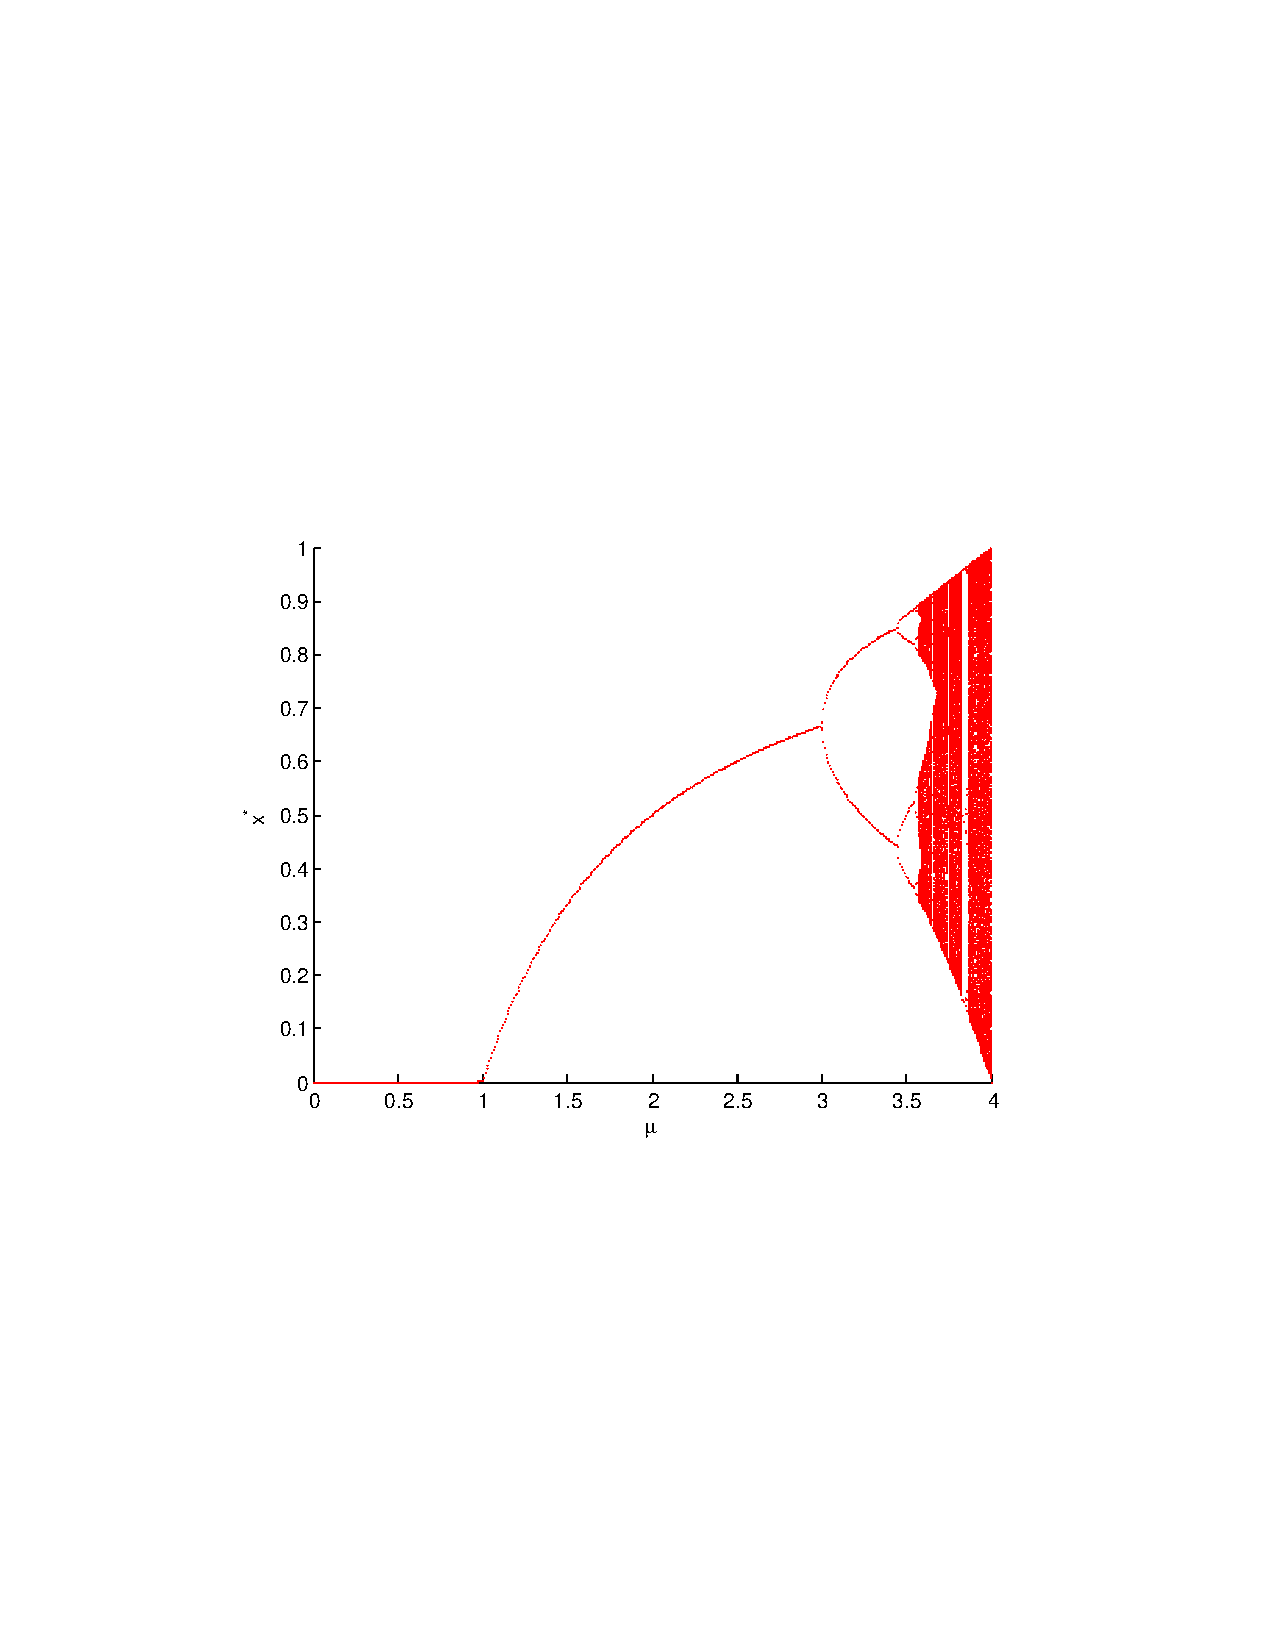
\includegraphics[width=0.5\textwidth]{cascade_full}
\end{center}
\caption{The cascade of bifurcation to chaos for the logistic growth.}
\end{figure}


{\bf Examples: Tumor cell growth }


A population of tumor cells $N(t)$ growing in a container can be modeled by a logistic growth
$$N(t+1)=rN(t)(1-N(t))$$
$r$ is the rate of growth of the tumor cells. Normalization of $N(t)$ means that $N(t)$ represents the fraction of the total population of cells contained in the cell culture. The cell culture can support a maximal number of cells represented by 1. The main assumption of the model is that the growth rate is constant.


\subsubsection{Other examples of population models exhibiting chaotic behaviors}


{\bf Ricker model }
another model for describing a population $N(t)$ in a limited environment
$$N(t+1)=N(t)\exp\left (r (1-\frac{N(t)}{K}) \right )=f(N(t))$$
where $r$ is the intrinsic growth rate and $K$ is the carrying capacity. The growth rate $f(N(t))$ is increasing  in $N(t)$ and the per capita growth $\frac{f(N)}{N}$ is decreasing in $N(t)$. The increase in population is not sufficient to compensate for the decrease in the per capita growth, then $\lim_{N(t)\rightarrow +\infty}f(N(t))=0$. Then the Ricker model can be referred as to overcompensatory.
\begin{itemize}
\item $r < 2$ Globally asymptotically stable equilibrium $\bar x=K$
\item r = 2 Bifurcation into a stable 2-cycle
\item r = 2.5 Bifurcation into a stable 4-cycle
\item Then there is a series of cycle duplication: 8-cycle, 16-cycle, etc.
\item r = 2.692 Chaos 
\item For $r > 2.7$ there are some regions where dynamics returns to a cycle, e.g., r=3.15. 
\end{itemize}



{\bf Hassell model}
a population $N(t)$ in a limited environment
$$N(t+1)=\frac{rN(t)}{(1 + N(t))^b}$$
where $r$ is the intrinsic growth rate for small populations and b represents the inhibitive density-dependent feedback, usually attributed to the environment. 



%{\bf Beverton-Holt model}
%$$N(t+1)=\frac{ e ^r K N(t)}{K + (e^r -1)N(t)}$$
%with $r$ is the intrinsic growth rate, the carrying capacity is $K$.

\subsection{Example of a 2-dimensional system}
\begin{equation*}
\begin{array}{cl}
x(t+1)=&x(t)(a-x(t)-y(t)), \quad a>0\\
y(t+1)=&y(t)(b+x(t)), \quad 0<b<1.
\end{array}
\end{equation*}


{\bf Equilibria: }
To find equilibria, solve for $x$ and $y$
\begin{equation*}
\begin{array}{cl}
x=&x(a-x-y)\\
y=&y(b+x)
\end{array}
\end{equation*}
Then, we found 3 equilibria:
$$(\bar x_1, \bar y_1)=(0,0), \quad  (\bar x_2, \bar y_2)=(a-1,0), \quad (\bar x_3, \bar y_3)=(1-b,a+b-2).$$

{\bf Local asymptotic stability of equilibrium: }
The Jacobian of the system is
$$
J=\left ( 
\begin{array}{cc}
a-2x-y & -x \\
y & b+x
\end{array}
\right )
$$
The Jacobians evaluated at each equilibrium are:
$$
J_{(\bar x_1, \bar y_1)}=\left ( 
\begin{array}{cc}
a & 0 \\
0 & b
\end{array}
\right ) \quad 
J_{(\bar x_2, \bar y_2)}=\left ( 
\begin{array}{cc}
2-a & 1-a \\
0 & b+a-1
\end{array}
\right ) \quad
J_{(\bar x_3, \bar y_3)}=\left ( 
\begin{array}{cc}
b & -1+b \\
a+b-2 & 1
\end{array}
\right )
$$
\begin{itemize}
\item Eigenvalues of $J_{(\bar x_1, \bar y_1)}$ are $a$ and $b$. By definition $|b|<1$. If $a<1$, $(\bar x_1, \bar y_1)$ is L.A.S.
\item $(\bar x_2, \bar y_2)=(a-1,0)$ exists only if $1<a$. Eigenvalues of $J_{(\bar x_2, \bar y_2)}$ are $2-a$ and $b+a-1$, then the stability of $(\bar x_2, \bar y_2)$ depends on $|2-a|<1$ and $|b+a-1|<1$. These inequalities lead to $1<a<2-b$.
\item From Theorem \ref{theo:stable2dim}, $(\bar x_3, \bar y_3)$ is L.A.S. if 
$$|1+b|<1+b-(-1+b)(a+b-2)<2.$$
$(\bar x_3, \bar y_3)$ is positive if $b<1$ and $a+b>2$. Then the biological existence and the LAS of $(\bar x_3, \bar y_3)$ are possible for
$$2<a+b<3.$$
\end{itemize}


\subsection{Epidemic models}
To study the spread of a disease in a population.




The population can be 
\begin{itemize}
\item closed (no immigration, no emigration, death and birth are neglected). 
\item open
\item homogeneous and homogeneously mixed (or not)
\end{itemize}
The population has a structure
\begin{itemize}
\item classification of individuals according to their disease status
\begin{itemize}
\item susceptible (S): individuals not infective but who are capable of contracting the disease
\item latent or exposed (E): infected by the disease, but not yet infectious
\item infective (I): infectious individual; an individual can be infectious before symptoms appear.
\item removed (R): no longer infectious, whether by acquiring immunity or death...
\item carrier: in some diseases, individual can remain infectious for long periods (e.g. for life), but do not show any symptoms of the disease themselves.
\end{itemize}
\item age
\item sex
\end{itemize}
Types of models
\begin{itemize}
\item SI model: no recovery.
\item SIS model: recovery but no immunity.
\item SIR model: recovery with permanent immunity.
\item SIRS model: recovery with temporary immunity.
\item ...
\end{itemize}
Parameters:
\begin{itemize}
\item $\beta$ transmission rate
\item $b$ rate of a birth
\item $d$ rate of death 
\item $\gamma$ rate of recovery; $1/\gamma $ is the average length of the infectious period when there are no death.
\item $1/(\gamma +b)$ is the average length of the infectious period when deaths are included.
\item $\nu$ rate of loss of immunity; $1/\nu$ average length of immunity.
\end{itemize}

\begin{definition}
The incidence is the rate at which infections occur. The incidence function is defined as $f(I,S)=\lambda(I)S$ where $\lambda(I)$ is the force of infection (probability of a given susceptible contracts the disease).
\end{definition}
Some incidence functions
\begin{itemize}
\item Mass action: infectives and susceptible mixed completely with each other, $f(I,S)=\beta IS$.
\item Proportional incidence (pseudo mass action): $f(I,S)=\beta \frac{I}{N}S$
\item Refuge effect: $$f(I,S)=\left \{\begin{array}{cc}\beta I (N-I/q)& I <qN\\
0 & I\geq qN\end{array}\right .$$
where $0<q<1$ is the proportion of population potentially suceptible because of spatial or other heterogeneities.
\item For vector-borne disease: Criss-cross infection (the vector infecting the host and the host then infecting another vector)
\item ...
\end{itemize}

\begin{definition}
The prevalence of a disease in a population is the fraction infected.
\end{definition}

\begin{definition}
The basic reproduction number $\mathcal{R}_0$ is the average number of secondary infections caused by one infectious individual in a totally susceptible population during the individual's infectious period.
\end{definition}
\begin{figure}[h]
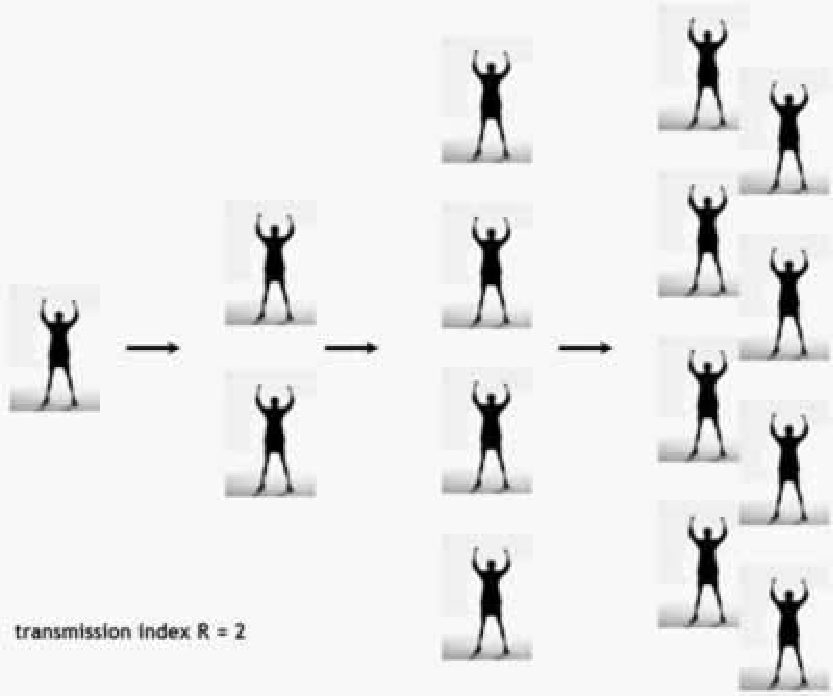
\includegraphics[width=.8\textwidth]{rzero}
\caption{Reproduction number $\mathcal{R}_0=2$.}
\end{figure}
Magnitude of the basic reproductive number gives an indication of the difficulty in controlling an epidemic or eradicating the disease: the larger the value of $\mathcal{R}_0$, the harder it is to control.

\subsubsection{SIR Model}
An example of SIR model using the difference equation formalism.
\begin{figure}[h]
\includegraphics[width=0.8\textwidth]{SIR}
\caption{SIR model: disease with recovery and permanent immunity, here birth=death=b.}
\end{figure}
$$
\begin{array}{cc}
S(t+1)=&S(t)-\beta \dfrac{S(t)}{N}I(t) +b(I(t)+R(t))\\
I(t+1)=&(1-\gamma -b)I(t)+\beta \dfrac{S(t)}{N}I(t)\\
R(t+1)=& R(t)(1-b)+\gamma I(t)
\end{array}
$$
where $N=S(0)+I(0)+R(0)$, parameters are:
\begin{itemize}
\item $\beta$ contact number, the average number of successful contacts made by one infected individual during the time $t$ and $t+1$
\item $b=$ rate of a birth = rate of death 
\item $\gamma$ rate of recovery; $1/\gamma $ is the average length of the infectious period when there are no death.
\item $1/(\gamma +b)$ is the average length of the infectious period when deaths are included.
%\item $\nu$ rate of loss of immunity; $1/\nu$ average length of immunity.
\end{itemize}
\begin{itemize}
\item  Population is constant: $N=S(t)+I(t)+R(t)$.
\item  Nonnegative solutions, if $b, \gamma >0$ and
$$0<b+\gamma <1, \qquad 0<\beta <1$$.
\item Reduced system: $R(t)=N-I(t)-S(t)$
$$
\begin{array}{cc}
S(t+1)=&S(t)-\beta \dfrac{S(t)}{N}I(t) +b(N-S(t))\\
I(t+1)=&(1-\gamma -b)I(t)+\beta \dfrac{S(t)}{N}I(t)
\end{array}
$$
\item Two equilibria: disease-free equilibrium $(S_1,I_1)=(N,0)$; 

and endemic equilibrium $(S_2,I_2)=\left (N\frac{(\gamma+b)}{\beta},bN\frac{\beta - (\gamma + b)}{\beta (\gamma +b)}\right )$
\item {\bf Stability at disease free equilibrium $(S_1,I_1)$}

The Jacobian evaluated at $(S_1,I_1)$ is
$$
J(S_1,I_1)=\left (
\begin{array}{cc}
1-b & -\beta \\
0 & 1-b-\gamma +\beta 
\end{array}
\right )
$$
as the Jacobian is upper triangular its eigenvalues are
$$\lambda _1 = 1-b , \quad \lambda _2= 1-b-\gamma +\beta  .$$
$(S_1,I_1)$ is locally asymptotically stable if $|\lambda_{1,2}|<1$
\begin{itemize}
\item from assumptions, we have $0<\lambda _1 <1$
\item if $\frac{\beta}{\gamma +b}<1$ (where $\mathcal{R}_0=\frac{\beta}{\gamma +b}$ is the basis reproduction number), $0<\lambda _2 <1$
\end{itemize}
\item if $\mathcal{R}_0 <1$, there exist only one (biologically plausible) equilibrium, the disease-free equilibrium, and it is L.A.S. (see Figure \ref{fig:SIRsimul})
\item {\bf Stability of the endemic equilibrium $(S_2,I_2)$}

The Jacobian evaluated at $(S_2,I_2)$ is
$$
J(S_2,I_2)=\left (
\begin{array}{cc}
1-b\mathcal{R}_0 & -\beta/\mathcal{R}_0 \\
b(\mathcal{R}_0-1) & 1
\end{array}
\right )
$$
where $\tr(J(S_2,I_2))=2-b\mathcal{R}_0 $ (assume $ \tr(J(S_2,I_2))\geq 0$), and $\det(J(S_2,I_2))=1-b\mathcal{R}_0+\beta b (1-\frac{1}{\mathcal{R}_0})$.


Condition for L.A.S (Theorem \ref{theo:stable2dim})
$$2-b\mathcal{R}_0 <2-b\mathcal{R}_0+\beta b (1-\frac{1}{\mathcal{R}_0}) <2$$
this condition is satified because
$$\beta (1-1/\mathcal{R}_0)<1<\mathcal{R}_0$$
\item If $1<\mathcal{R_0}\leq 2/b$, the endemic equilibrium  exists and it is L.A.S. (see Figure \ref{fig:SIRsimul}).
\end{itemize}
\begin{figure}[h]
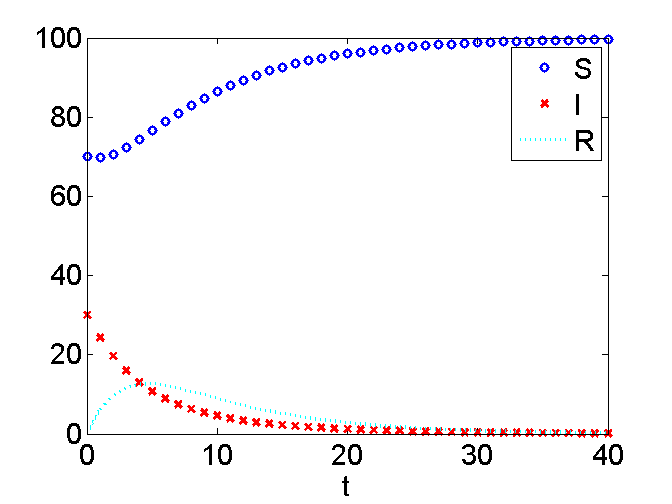
\includegraphics[width=.49\textwidth]{R1}
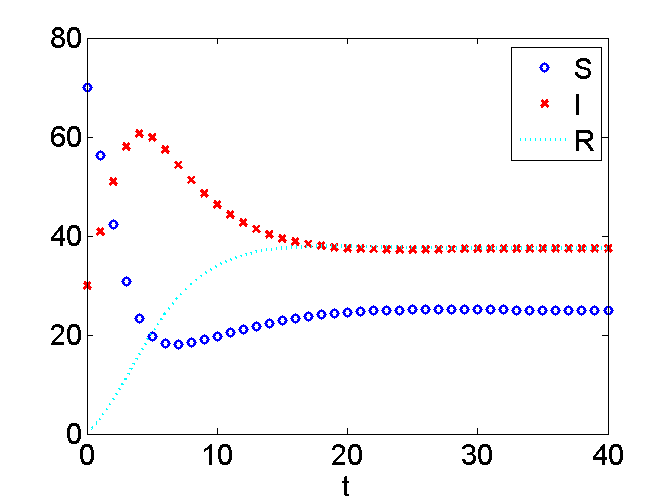
\includegraphics[width=.49\textwidth]{R4}
\label{fig:SIRsimul}
\caption{SIR model: {\bf Left)} $R_0=0.75$ the disease-free equilibrium is L.A.S. {\bf Right)} $R_0=4$ the endemic equilibrium is L.A.S}
\end{figure}

\subsection{Predator-Prey models}
{\bf Assumptions}
\begin{itemize}
\item the prey has unlimited resources
\item the prey's only threat is the predator
\item the predator is a specialist; i.e., the predator's only food supply is the prey
\item predator growth depends on the prey it catches
\end{itemize}
{\bf Variables}
\begin{itemize}
\item $N(t)$ number of preys
\item $P(t)$ number of predators
\end{itemize}
{\bf Parameters}
\begin{itemize}
\item $r$ intrinsic rate of growth of prey
\item $d$ rate of death of predators
\item $eP(t)$ per capita prey reduction due to predation
\item $bN(t)$ per capita predator increase due to prey
\end{itemize}
\begin{equation*}
\begin{array}{cl}
N(t+1)=&(1+r)N(t)-e N(t)P(t)\\
P(t+1)=&(1-d)P(t)+bN(t)P(t)
\end{array}
\end{equation*}

{\bf Neubert and Kot model:}
If the prey follows a logistic growth
\begin{equation*}
\begin{array}{cl}
N(t+1)=&N(t)+rN(t)\left ( 1-\frac{N(t)}{K} \right ) -e N(t)P(t)\\
P(t+1)=&(1-d)P(t)+bN(t)P(t)
\end{array}
\end{equation*}

\part{Differential equations}
\section{Ordinary differential equations}



\begin{definition}
The standard form of first order linear
equations is
$$\frac{dy}{dt}+p(t)y=g(t)$$
$p$ and $g$ are given functions of the independent variable $t$.
\end{definition}



\vspace{1cm}

Let define a system of $n$ autonomous differential equations
\begin{equation}\label{eq:ODEGeneral}
\frac{dY}{dt}=F(Y)
\end{equation}
where $Y=(y_1,y_2,\dots,y_n)^T$ and $F(Y)=(f_n(y_1,\dots,y_n),\dots,f_n(y_1,\dots,y_n))^T$, and $F$ does not depend explicit on $t$.
\begin{definition}
An equilibrium solution of equation \eqref{eq:ODEGeneral} is a constant solution $\bar Y$ satisfying $$F(\bar Y)=0.$$
\end{definition}

\begin{definition}(Locally stable)
An equilibrium solution $\bar Y$ of \eqref{eq:ODEGeneral} is said to be locally stable if for each $\epsilon>0$ there exits a $\delta >0$ such that every solution $Y(t)$ of \eqref{eq:ODEGeneral} with the initial condition $Y(t_0)=Y_0$,
$$\| Y_0-\bar Y\| _2< \delta,$$
satisfies the condition that
$$\| Y(t)-\bar Y\| _2< \epsilon$$
for all $t \geq t_0$.

If the equilibrium solution is not locally stable it is said to be unstable.
\end{definition}

Euclidian distance between two points $Y_1=(y_1^1,y_2^1,\dots,y_n^1)$ and $Y_2=(y_1^2,y_2^2,\dots,y_n^2)$ in $\mathbb{R}^n$ is $$\|Y_1-Y_2\|_2=\sqrt{\sum _{i=1}^n(y_i^1-y_i^2)^2}.$$

\begin{definition}(Locally asymptotically stable) 
An equilibrium solution $\bar Y$ of \eqref{eq:ODEGeneral} is said to be locally asymptotically stable if it is locally stable and if there exist $\gamma >0$ such that $\| Y_0-\bar Y\| _2< \gamma$ implies
$$\lim_{t\rightarrow \infty}\| Y(t)-\bar Y\| _2=0.$$
\end{definition}


\begin{definition}(Periodic solution)
A periodic solution of the system \eqref{eq:ODEGeneral} is a nonconstant solution $Y(t)$ satisfying $Y(t+T)=Y(t)$ for all $t$ on the interval of existence  for some $T>0$. The minimum value of $T$ is called the period of the solution.
\end{definition}

\subsection{First order differential equations}
\subsubsection{Analytical methods}


{\bf Linear equations: Integrating factors}



To solve $1^{st}$ order linear equation with non-constant coefficients (this method can also be used for equation with constant coefficient).
\begin{enumerate}
\item Put the DE in the standard form
\begin{equation}\frac{dy}{dt}+p(t)y=g(t)\label{eq:DE}\end{equation}
\item Determine the integrating factor $\mu (t)$
\begin{itemize}
\item Multiply the DE (\ref{eq:DE}) by $\mu (t)$
\begin{equation}\mu (t)\frac{dy}{dt}+\mu (t)p(t)y=\mu
(t)g(t)\label{eq:DE1}\end{equation} 
\item  State that the left side of (\ref{eq:DE1}) is equal to $\frac{d}{dt}(\mu (t)y)$
$$\frac{d}{dt}(\mu (t)y)=\mu (t)\frac{dy}{dt}+y\frac{d \mu}{dt}=\mu (t)\frac{dy}{dt}+\mu
(t)p(t)y$$
\item Solve for $\mu (t)$
$$\frac{d \mu }{dt}=\mu (t) p(t)$$
\end{itemize}
$$\Rightarrow \quad \mu(t)=e^{\int p(t)dt}$$
\item Solve (\ref{eq:DE1}) for $y$ with $\mu(t)=e^{\int p(t)dt}$
$$\left(\frac{d}{dt}e^{\int p(t)dt}y=\right)e^{\int p(t)dt}\frac{dy}{dt}+p(t)e^{\int p(t)dt}y=e^{\int p(t)dt}g(t)$$
$$\frac{d}{dt}\mu(t)y=\mu(t)g(t)$$
$$\mu(t)y=\int \mu(t)g(t)dt +c$$
\end{enumerate}

Hence the general solution of (\ref{eq:DE}) is
$$y(t)=\frac{1}{\mu(t)}\left [\int_{t_0}^t \mu(s)g(s)ds +c\right ]
\quad with \quad \mu(t)=e^{\int p(t)dt}$$




{\bf Separable equations}



\begin{definition}(Separable equations) A first order differential equation
$$\frac{dy}{dx}=f(x,y)$$
is said to be separable or to have separable variables if it can be
expressed as follows
$$\frac{dy}{dx}=g(x)h(y)$$
(the rate function can be expressed as a product of a function of
the independent variable times a function of the dependent variable
).
\end{definition}


{\bf To solve separable equations: }
$\frac{dy}{dx}=g(x)h(y)$
\begin{enumerate}
\item Express the separable equation as follows
$$\frac{1}{h(y)}\frac{dy}{dx}=g(x)$$
\item As $y$, $\frac{dy}{dx}$, and $g(x)$ are functions of $x$,
apply the integral
$$\int \frac{1}{h(y)}\frac{dy}{dx} dx=\int g(x) dx$$
\item Use the Change of variable Theorem (if $u=v(x)$ $\int f(v(x))v'(x)dx=\int
f(u)du$) for the left side with $u=y(x)$
$$\int \frac{1}{h(u)}du=\int g(x) dx$$
$$\int \frac{1}{h(y)}dy=\int g(x) dx$$
\item Integrate
\begin{equation}H(y)=G(x)+c\label{eq:GS}\end{equation} $c$ is the combination of the left
and right integration constants, $H$ and $G$ are antiderivatives of
$\frac{1}{h(y)}$ and $g(x)$ respectively. \item Solve equation
(\ref{eq:GS}) for $y$ to obtain a explicit form of the general
solution.
\end{enumerate}



\subsubsection{Local stability}
A simple criterion for determining the L.A.S. of an equilibrium solution to a first order autonomous differential equation
\begin{equation}
\label{eq:ODE1Nonlin}
\frac{dy}{dt}=f(y)
\end{equation}
having an equilibrium at $\bar y$.


\begin{theorem}
Suppose $f'$ is continuous on an open interval $I$ containing $\bar y$, where $\bar y$ is an equilibrium of $\frac{dy}{dt}=f(y)$. Then $\bar y$ is locally asymptotically stable if $$f'(\bar y)<0$$
and unstable if $f'(\bar y)>0$.
\end{theorem}

The value $f'(\bar y)$ is know as the eigenvalue of the linearized equation.


\begin{definition}
The equilibrium $\bar y$ of $\frac{dy}{dt}=f(y)$ is called hyperbolic if $f'(\bar y)\not =0$. Otherwise, it is called nonhyperbolic.
\end{definition}


Nonhyperbolic equilibria have a zero eigenvalue, and hence their local stability is indeterminate.


\subsubsection{Phase line analysis}
Consider a first-order nonautonomous equation
$$\frac{dy}{dt}=f(t,y).$$
$f(t,y)$ represents the slope of the tangent to the solution $y(t)$ at the point $(t,y)$. Hence $f(t,y)$ can be used to construct a direction field in the $t,y-$plane.

Consider a first-order autonomous equation
$$\frac{dy}{dt}=f(y).$$
Here the direction of flow does not change with $t$. Hence it is only necessary to determine the direction of flow on the $y-$axis (Phase line). If $\frac{dy}{dt}$ is positive, the direction of flow is in the positive direction, if it is negative, the flow is in negative direction.



\subsection{Higher-order linear equations}
The general solution to an $n^{th}-$order linear nonhomogeneous differential equation is the sum of two solutions, a general solution to the homogeneous differential equation and a particular solution to the nonhomogeneous differential equation
$$y(t)=y_h(t)+y_p(t).$$ 



{\bf $\bullet$} Methodology to find the general solution to the homogeneous equation is given for second-order linear equations, but it can be generalized to the $n^{th}-$order linear equations.


\begin{theorem} (Principle of superposition)
If $y_1$ and $y_2$ are two solutions of the homogeneous linear differential
equation on an interval $I$


$$y''+p(t)y'+q(t)y=0$$

then the linear combination $$c_1y_1+c_2y_2$$ is also a solution for
any values of the constants $c_1$ and $c_2$ on the interval.
\end{theorem}

\begin{definition}(Wronskian)
Suppose each of the functions $f_1(t),
f_2(t), \dots, f_n(t)$ has at least $n-1$ derivatives. The
determinant

$$W(f_1,f_2,\dots,f_n)=\left |
\begin{array}{llll}
f_1 & f_2 & \cdots & f_n\\
f_1' & f_2' & \cdots & f_n'\\
\vdots & \vdots & &\vdots\\
f_1^{(n-1)} & f_2^{(n-1)} & \cdots & f_n^{(n-1)}\\
\end{array}
\right |$$ is called the Wronskian of the functions.
\end{definition}


\begin{theorem}
Let $y_1$ and $y_2$ be solutions of the differential equation
$$
y''+p(t)y'+q(t)y=0$$ where $p$ and $q$ are continuous on an open
interval $I$. Then $y_1$ and $y_2$ are linearly independent on $I$
if and only if $W(y_1,y_2)(t)\not=0$ $\forall t \in I$.
\end{theorem}

\begin{definition}
Any set $y_1$, $y_2$ of 2 linearly independent solutions of
$$
y''+p(t)y'+q(t)y=0$$ on an open interval $I$ is said to be {\bf a
fundamental set of solutions} on $I$ of the differential equation.
\end{definition} 


\begin{definition}
The general solution of
$$y''+p(t)y'+q(t)y=0$$ on an open interval $I$ is the linear combination of 2 linearly independent solutions $y_1$ and $y_2$
$$y(t)=c_1 y_1(t)+c_2y_2(t)$$
with $c_1$ and $c_2$ constants. $y_1$ and $y_2$ form a fundamental set of solutions.
\end{definition}


{\bf Method for linear homogeneous
second-order equations with constant coefficients}
\begin{equation}
ay''+by'+cy=0\label{eq:constant}
\end{equation}
Let assume that the solution can take the form of $$y(t)=e^{rt}.$$
\vspace{-.2cm}
 \begin{enumerate}
\item Write the {\bf characteristic equation }
$$ar^2+br+c=0$$
\item Find the {\bf roots} $r_1$ and $r_2$ of the characteristic equation
$$r_1=\frac{-b-\sqrt{\Delta}}{2a} , \qquad r_2=\frac{-b+\sqrt{\Delta}}{2a}, \quad \textrm{with} \quad \Delta=b^2-4ac $$
\begin{description}
\item[$\Delta >0$]: $r_1$, $r_2$ distinct and real,
$y_1(t)=e^{r_1t}$ and $y_2(t)=e^{r_2t}$ are 2 linearly independent
solutions of \eqref{eq:constant}. The general solution is
$$y(t)=c_1 e^{r_1t}+c_2e^{r_2t}, \quad c_1, c_2\textrm{ arbitrary constants}$$
\item[$\Delta =0$]: $r_1=r_2=r$ real, $y_1(t)=e^{rt}$ and $y_2(t)=te^{rt}$ are 2 linearly independent
solutions of \eqref{eq:constant}. The general solution is
$$y(t)=c_1 e^{rt}+c_2te^{rt} , \quad c_1, c_2\textrm{ arbitrary constants}$$
\item[$\Delta <0$]: $r_1$, $r_2$ complex conjugates, $r_1=\alpha + i \mu$ and $r_2=\alpha - i
\mu$. $y_1(t)=e^{\alpha t}\cos (\mu t)$ and $y_2(t)=e^{\alpha t}\sin
(\mu t)$ are 2 linearly independent solutions of
\eqref{eq:constant}. The general solution is
$$y(t)=c_1 e^{\alpha t}\cos (\mu t)+c_2e^{\alpha t}\sin (\mu t) , \quad c_1, c_2\textrm{ arbitrary constants}$$
\end{description}
\end{enumerate}

Note that an $n^{th}-$order linear homogeneous differential equation always has a solution equal to zero $y(t)\equiv 0$. When the equation has constant coefficients, the stability of the zero solution is stable (when a solution to an IVP will tend to zero). Stability of the zero solution depends on the eigenvalues, the roots of $\lambda_i$ of the characteristic equation.

\begin{theorem}
If all of the roots of the characteristic polynomial $P(\lambda)$ are negative or have negative real part, then given any solution $y(t)$ of the homogeneous differential equation $$\frac{d^n y}{dy^n}+a_1(t)\frac{d^{n-1}y}{dy^{n-1}}+\dots+a_{n-1}(t)\frac{dy}{dy}+a_n(t)y=0,$$ there exist positive constant $M$ and $b$ such that
$$|y(t)|\leq Me^{-bt}\quad for \quad t>0$$
and
$$\lim _{t\rightarrow \infty} |x(t)|=0$$
\end{theorem}




Methodologies to find a particular solution to the nonhonogeneous differential equation:
\begin{itemize}
\item Undetermined coefficients
\item Variation of parameters
\end{itemize}


{\bf Undetermined coefficients (to find
a particular solution $Y(t)$)}
\begin{itemize}
\item Make an assumption about the form of the particular solution
$Y(t)$ but with the coefficients unspecified
\item The particular solution has to satisfy the nonhomogeneous
equation $\Leftrightarrow$ Substitute the assumed expression of
$Y(t)$ in the nonhomogeneous equation $\Rightarrow$ Coefficients to
be determined
\end{itemize}
Conditions for application: 
if $g(t)$ takes the form: constant function, exponential, polynomial, sine, cosine, any sum or products of such functions.
$$y''+p(t)y'+q(t)y=g(t)$$
\begin{itemize}
\item Make an assumption about the form of the particular solution
 $Y(t)$: if $g(t)$ is of the form in the left column or is the sum or product of such function, then check a particular solution $Y(t)$ of the corresponding form as indicated in the right column

\begin{tabular}{l|l}
$\mathbf{g(t)}$ & {\bf Assumed form of }$Y(t)$\\
$\alpha e^{\beta t}$& $ae^{\beta t}$\\
$\alpha \cos (\omega t) +\beta \sin (\omega t)$ & $a \cos (\omega t)
+b \sin (\omega t)$\\
$\alpha$ & $a$\\
$\alpha + \beta t$ & $a +bt$\\
$\alpha + \beta t +\gamma t^2$ & $a +bt +ct^2$\\
$\alpha + \beta t +\gamma t^2+ \cdots+\delta t^m$ & $a +bt +ct^2+ \cdots+d t^m$\\
\end{tabular}
\item If coefficients cannot be determined, then no solution of this
form exists $\Rightarrow$ modify the assumption
\item If $g(t)$ contains terms that duplicate any solutions of the corresponding homogeneous equation
$\Rightarrow$ each such term must be multiplied by $t^s$
($s$ the smallest natural number that eliminates the
duplication).
\end{itemize}


{\bf Variation of parameters: }
$y''+p(t)y'+q(t)y=g(t)$
\begin{enumerate}
\item Find the {\bf general solution of the homogeneous
equation} $\Leftrightarrow$ Find 2 linearly independent solutions
$y_1$ and $y_2$ of the homogeneous equation
\item Check for the nonhomogeneous equation a solution of the form
$$Y(t)=u_1(t)y_1(t)+u_2(t)y_2(t)$$
where $u_1$ and $u_2$ are two functions of $t$ to be determined, and
that satisfy the {\bf second condition}
$$u_1'(t)y_1(t)+u_2'(t)y_2(t)=0$$
\item Substitute $Y(t)$ in the nonhomogeneous equation and use the
second condition to obtain
$$u'_1(t)y_1'(t)+u_2'(t)y_2'(t)=g(t)$$
\item Solve  the system of 2 linear algebraic
equation for $u_1'$ and $u_2'$
$$\left \{
\begin{array}{ll}
u_1'(t)y_1(t)+u_2'(t)y_2(t)&=0\\
u'_1(t)y_1'(t)+u_2'(t)y_2'(t)&=g(t)
\end{array}\right . \mathrm{or} \quad
\left [
\begin{array}{ll}
y_1(t)&y_2(t)\\
y_1'(t)&y_2'(t)
\end{array}\right ]\left [
\begin{array}{l}
u_1'(t)\\
u_2'(t)
\end{array}\right ]=\left [
\begin{array}{l}
0\\
g(t)
\end{array}\right ]
$$

$$\Rightarrow u_1'(t)=\frac{-y_2(t)g(t)}{W(y_1,y_2)(t)}, \qquad u_2'(t)=\frac{y_1(t)g(t)}{W(y_1,y_2)(t)}$$
\item Integrate, evaluate the integral omitting the integration
constants
$$\Rightarrow u_1(t)=-\int \frac{y_2(t)g(t)}{W(y_1,y_2)(t)}dt, \qquad u_2(t)=\int \frac{y_1(t)g(t)}{W(y_1,y_2)(t)}dt$$
\item A {\bf particular solution} of the nonhomogeneous equation is
$$Y(t)=-y_1(t)\int \frac{y_2(t)g(t)}{W(y_1,y_2)(t)}dt + y_2(t)\int \frac{y_1(t)g(t)}{W(y_1,y_2)(t)}dt$$
\item The {\bf general solution} of the nonhomogeneous equation is
$$y(t)=c_1y_1(t)+c_2y_2(t)+Y(t), \qquad c_1, \; c_2 \; \textrm{arbitrary constants}$$
\end{enumerate}


\begin{theorem}
If the functions $p$, $q$ and $g$ are continuous on an open interval
$I$, and if the functions $y_1$ and $y_2$ are linearly independent
solutions of the homogeneous equation, $y''+p(t)y'+q(t)y=0$,
corresponding to the nonhomogeneous equation
$$y''+p(t)y'+q(t)y=g(t)$$
then a particular solution of the nonhomogeneous equation is
$$Y(t)=-y_1(t)\int_{t_0}^t \frac{y_2(s)g(s)}{W(y_1,y_2)(s)}ds+y_2(t)\int_{t_0}^t \frac{y_1(s)g(s)}{W(y_1,y_2)(s)}ds$$
where $t_0$ is any point in $I$. The general solution is
$$y(t)=c_1y_1(t)+c_2y_2(t)+Y(t).$$
\end{theorem}

\subsection{Systems of equations}
\subsubsection{Systems of linear equations}
A $n-$dimensional linear system
$$\frac{dX}{dt}=A X$$
where $A$ is a $n\times n$ constant matrix with real elements. The general solution of this system is
$$X(t)=e^{At}C$$
where $e^{At}$ is a $n\times n$ matrix known as the fundamental matrix and $C$ ia a $n\times 1$ vector. There exist many methods to compute the matrix exponential. To compute the general solution of the $n-$dimensional system, a straightforward method can be used (similar method used for higher-order constant coefficient DE).




Here the case of a 2-dimensional linear system is studied. 
Consider a system of first-order linear equations
\begin{equation}
\frac{dX}{dt}=A X
\label{eq:SysLin}
\end{equation}
where $X=(x_1,x_2)^T$ and $A$ is a constant $2\times 2$ matrix. Note that the zero solution $X=0$ is solution of the differential equation. 

Let $X=e^{\lambda t}V$ be a solution of \eqref{eq:SysLin}, then
$$AV=\lambda V$$
where $\lambda $ is the eigenvalue of $A$ and $V$ is the eigenvector corresponding to $\lambda$. The eigenvalues are solutions of $$\det (A-\lambda I)=0.$$
Then
$$\lambda ^2 -\tr (A) \lambda + \det (A)=0.$$
Solutions of \eqref{eq:SysLin} can take 3 different forms
\begin{itemize}
\item if eigenvalues are real and distinct
$$X(t)=c_1V_1 e^{\lambda _1t}+c_2V_2 e^{\lambda _2t}$$
with $c_1$ and $c_2$ constant.
\item if eigenvalues are real and equal
$$X(t)=c_1V_1 e^{\lambda _1t}+c_2\left (V_1te^{\lambda _1t}+P e^{\lambda _1t}\right )$$
with $c_1$ and $c_2$ constant. $P$ can be obtained by solving $(A-\lambda _1 I)P=V_1$.
\item if eigenvalues are complex conjugate $\lambda _{1,2}=a\pm i b$
$$X(t)=P_1 e^{at} \cos (bt) + P_2 e^{at}\sin (bt).$$
\end{itemize}
Behaviors of solutions:
\begin{itemize}
\item The origin is asymptotically stable if the eigenvalues of $A$ are negative or have negative real part.
\item The origin is stable if the eigenvalues of $A$ are nonpositive or have nonpositive real part.
\item The origin is unstable if the eigenvalues of $A$ are positive or have positive real part.
\end{itemize}


\begin{theorem}
Suppose $\frac{dX}{dt}=A X$ where $A$ is a constant $2\times 2$ matrix with $\det (A) \not =0$. 

The orign is asymptotically stable iff
$$\tr(A)<0 \quad and \quad \det (A)>0.$$

The orign is stable iff
$$\tr(A)\leq 0 \quad and \quad \det (A)>0.$$


The origin is unstable iff 
$$\tr(A)> 0 \quad or \quad \det (A)<0.$$
\end{theorem}


In the case of real eigenvalues $\lambda _1$ and $\lambda _2$, the eigenvectors $V_1$ and $V_2$ are directions along which solutions travel toward or away the origin:
\begin{itemize}
\item if $\lambda _1$ is positive, solutions will travel along $V_1$ away from the origin.
\item if $\lambda _2$ is negative, solutions will travel along $V_2$ toward the origin.
\end{itemize}
Hence solutions travel in a direction which corresponds to a linear combination of $V_1$ and $V_2$
\begin{theorem}
Consider a system of first order linear equations
$$\frac{dX}{dt}=A X$$
where $X=(x_1,x_2)^T$ and $A$ is a $2\times 2-$matrix.
\begin{itemize}
\item if $\det A >0$ and $\tr A ^2 -4 \det A\geq 0$ then the origin is a node (real eigenvalues having the same signs); a stable node if $\tr A <0$ (real $\lambda _{1,2}<0$), and an unstable node if $\tr A >0$ (real $\lambda _{1,2}>0$).
\item if $\det A <0$ then the origin is a saddle (real eigenvalues have opposite signs, $\lambda _1 \lambda _2<0$).
\item if $\det A >0$ and $\tr A ^2 -4 \det A < 0$ and $\tr A \not =0$, the origin is a spiral (complex conjugate with nonzero real part); it is stable if $\tr A <0$ (negative real part) and unstable if $\tr A >0$ (positive real part).
\item if $\det A >0$ and $\tr A=0$ then the origin is a center (purely imaginary eigenvalues $\lambda _{1,2}=\pm ib$).
\end{itemize}
\end{theorem}


\subsubsection{Tools to determine properties of eigenvalues}
\begin{theorem}(Routh-Hurwitz Criteria)
Given the polynomial,
$$P(\lambda)=\lambda ^n + a_1 \lambda ^{n-1}+\dots + a_{n-1}\lambda +a_n$$
where the coefficients $a_i$ are real constants, $i=1,\dots , n$ define the $n$ Hurwitz matrices using the coefficients $a_i$ of the characteristic polynomial:
$$H_1=(a_1),\quad H_2=\left (\begin{array}{cc}a_1 & 1 \\ a_3 &a_2\end{array}\right), \quad H_3=\left (\begin{array}{ccc}a_1 & 1 & 0 \\ a_3 &a_2 &a_1 \\ a_5& a_4 & a_3\end{array}\right),$$
and
$$H_n=\left (\begin{array}{cccccc}a_1 & 1 & 0 & 0 & \dots &0\\ a_3& a_2 & a_1 & 1 & \dots & 0 \\ a_5 & a_4 & a_3 & a_2 & \dots &0\\\vdots & \vdots & \vdots & \vdots & \dots & \vdots \\ 0 & 0& 0& 0& \dots & a_n\end{array}\right )$$
where $a_j=0$ if $j>n$. All of the roots of the polynomial $P(\lambda)$ are negative or have negative real part if and only if the determinants of all Hurwitz matrices are positive:
$$\det H_i>0, \quad j=1,2,\dots, n.$$
\end{theorem}



\begin{theorem}(Corollary)
Routh-Hurwitz criteria for $n=2,3,4,5$
\begin{itemize}
\item $n=2:$ $a_1>0$ and $a_2>0$.
\item $n=3:$ $a_1>0,$ $a_3>0$ and $a_1a_2>a_3$.
\item $n=4:$ $a_1>0,$ $a_3>0,$ $a_4>0$  and $a_1a_2a_3>a_3^2+a_1^2a_4$.
\item $n=5:$ $a_i>0,$ $i=1,2,3,4,5,$ $a_1a_2a_3>a_3^2+a_1^2a_4$ and $(a_1a_4-a_5)(a_1a_2a_3-a_3^2-a_1^2a_4)>a_5(a_1a_2-a_3)^2+a_1a_5^2$
\end{itemize}
\end{theorem}



\begin{theorem}(Gerhgorin's Theorem)
Let $A$ be an $n\times n$ matrix. Let $D_i$ be the disk in the complex plane with the center at $a_{ii}$ and radius $r_i=\sum _{j=1,j\not =i}^n|a_{ij}|$. Then all eigenvalues of the matrix $A$ lie in the union of the disks $D_i$, $i=1,2,\dots, n$, $\cup_{i=1}^nD_i$. In particular, if $\lambda $ is an eigenvalue of $A$, then for some $i=1,2,\dots,n$
$$|\lambda -a_{ii}|\leq r_i.$$
\end{theorem}

\begin{theorem}(Corollary)
Let $A$ be an $n\times n$ matrix with real entries. If the diagonal elements of $A$ satisfy 
$$a_{ii}<-r_{i} \quad where \quad r_i=\sum _{j=1,j\not =i}^n|a_{ij}|$$
for $i=1,2,\dots,n$ then the eigenvalues of $A$ are negative or have have negative real part.
\end{theorem}



\subsubsection{Systems of nonlinear equations}
\begin{theorem}(Existence and Uniqueness)
Assume that $F$ and $\frac{\partial F}{\partial x_i}$ for $i=1,\dots, n$ are continuous functions of $(x_1,x_2,\dots , x_n)$ on $\mathbb{R}^n$. Then a unique solution exits to the initial value problem
$$\frac{dX}{dt}=F(X), \quad X(t_0)=X_0$$
for any initial value $X_0\in \mathbb{R}^n$.
\end{theorem}

\begin{theorem} (Hartman-Grobman)
Assume that $(\bar x, \bar y)$ is a hyperbolic (all eigenvalues of the Jacobian matrix evaluated at $(\bar x,\bar y)$ have nonzero real part) equilibrium. Then, in a small neighborhood of $(\bar x, \bar y)$, the nonlinear system 
behaves in a similar manner as the linearized system.
\end{theorem}


%Consider the first-order autonomous differential equation
%$$
%\begin{array}{ll}
%\frac{dx}{dt}=& f(x,y),\\
%\frac{dy}{dt}=& g(x,y).
%\end{array}
%$$
\begin{theorem}
Assume the first-order partial derivatives of $f$ and $g$ are continuous in some open set containing the equilibrium $(\bar x,\bar y)$ of the system
$$
\begin{array}{ll}
\frac{dx}{dt}=& f(x,y),\\
\frac{dy}{dt}=& g(x,y).
\end{array}
$$
Then the equilibrium is locally asymptotically stable if
$$\tr J <0 \quad and \quad \det J >0,$$
where $J$ is the Jacobian matrix evaluated at the equilibrium $(\bar x,\bar y)$. In addition, the equilibrium is unstable if either $\tr J >0$ or $\det J<0$.
\end{theorem}

As the linearization is only an approximation of the nonlinear system, the nonlinear system may behave differently from the linear system in 3 cases:
\begin{itemize}
\item $\det (J)=0$: there exists at least one zero eigenvalue, then the equilibrium in the nonlinear system may be a node, a saddle or a spiral.
\item $\tr(J)=0$ and $\det (J)>0$: eigenvalues are purely imaginary. The equilibrium in the nonlinear system may be a spiral or a center.
\item $\tr (J)^2=4\det (J)$: in the nonlinear system the equilibrium may be a node or a spiral.
\end{itemize}


Theorem for $n-$dimensional system:
\begin{theorem}
Suppose $dX/dt=F(X)$ is a nonlinear first-order autonomous system with an equilibrium $\bar X$. Denote the Jacobian matrix of $F$ evaluated at $\bar X$ as $J(\bar X)$. If the characteristic equation of the Jacobian matrix $J(\bar X)$,
$$\lambda ^n + a_1 \lambda ^{n-1}+\dots + a_{n-1}\lambda +a_n=0$$
satisfies the conditions of the Routh-Hurwitz criteria, that is, the determinants of all the Hurwitz matrices are positive $\det (H_j)>0$, $j=1,\dots,n$ then the equilibrium $\bar X$ is L.A.S. If $\det (H_j)<0$ for some $j=1,\dots , n$ then the equilibrium $\bar X$ is unstable.
\end{theorem}


{\bf Phase Plane analysis: }
To study the qualitative behavior of a system without solving it.
$$
\begin{array}{ll}
\frac{dx}{dt}=& f(x,y),\\
\frac{dy}{dt}=& g(x,y)
\end{array}
$$
Solutions curves (trajectories) $(x(t),y(t))$ are parametric equations with $t$ as an parameter.

At any point $(x,y)$, 
$$\frac{dy}{dx}=\frac{g(x,y)}{f(x,y)}$$
is the slope of the trajectory in the $xy-$plane and the tangent vector that gives the direction of the trajectory is $(f(x,y),g(x,y))$. The collection of vectors evaluated at any point of the $xy-$plane defines the direction field.


\begin{definition}
The $x-$nullcline for
$$
\begin{array}{ll}
\frac{dx}{dt}=& f(x,y),\\
\frac{dy}{dt}=& g(x,y)
\end{array}
$$
is the set of all points in the $xy-$plane satisfying $f(x,y)=0$.

The $y-$nullcline for
$$
\begin{array}{ll}
\frac{dx}{dt}=& f(x,y),\\
\frac{dy}{dt}=& g(x,y)
\end{array}
$$
is the set of all points in the $xy-$plane satisfying $g(x,y)=0$.
\end{definition}

At any intersection of $x-$nullcline and $y-$nullcline, there is an equilibrium point.

On the $x-$nullcline, all vectors are vertical. On the $y-$nullcline, all vectors are horizontal.
We need to check if the direction of flow is up or down on the $x-$nullcline, and if the direction of flow is left or right on the $y-$nullcline.

\subsection{Bifurcations}
Mathematical models have many parameters. When parameter values change, a change in the behavior of the solution can be expected. If the variation of a parameter change the qualitative behavior of the solution, there is a bifurcation.


Consider the differential equation
$$\frac{dx}{dt}=f(x,\mu), \quad x\in \mathbb{R} \quad \mu \in \mathbb{R}.$$
where $\mu$ is the parameter.

\begin{definition}
$\bar x$ is a bifurcation point and $\bar \mu$ is a bifurcation value if
$$f(\bar x, \bar \mu)=0, \quad \textrm{and} \quad \frac{\partial }{\partial x}f(\bar x, \bar \mu)=0.$$
\end{definition}


Different types of bifurcations in the case of scalar differential equations:
\begin{itemize}
\item Saddle-node bifurcation
\item Transcritical bifurcation
\item Pitchfork bifurcation
\end{itemize}
These types of bifurcations also occur in higher-dimensional system.

A fourth type of bifurcation can occurs in systems consisting of two or more equations: the Hopf bifurcation.

Consider a system of autonomous DEs:
\begin{align*}
\frac{dx}{dt}=&f(x,y,r)\\
\frac{dy}{dt}=&g(x,y,r)
\end{align*}
$f$ and $g$ depends on the parameter $r$. Assume that $(\bar x(r), \bar y(r))$ is an equilibrium and the Jacobian evaluated at this equilibrium has eigenvalues $\alpha(r)\pm i \beta (r)$.

A change of stability occurs at $r=\bar r$ where $\alpha (\bar r)=0$. If $\alpha (r)<0$ for $r<\bar r$ and $\alpha (r)>0$ for $r>\bar r$ (with $\beta (r)\not =0$), then the equilibrium changes from a stable spiral to an unstable spiral when $r$ passes through $\bar r$. The Hopf Theorem states that there is a periodic orbit near $r=\bar r$ from any neighborhood of the equilibrium is $\mathbb{R}^2$. Then $r$ is the parameter of bifurcation and the bifurcation value is $\bar r$.


\begin{theorem}(Hopf bifurcation)
Consider the system
\begin{align*}
\frac{dx}{dt}=&f(x,y,r)\\
\frac{dy}{dt}=&g(x,y,r)
\end{align*}
where $f(x,y,r)$ and $g(x,y,r)$ are continous and differentiable. The system has an equilibrium $(\bar x(r), \bar y(r))$, and the Jacobian of the system evaluated at this parameter-dependent equilibrium is $J(r)$. The Jacobian matrix $J(r)$ has eigenvalues $\alpha(r)\pm i \beta (r)$.

Assume that there exists a value $\bar r$ called the bifurcation value, such that $\alpha (\bar r)=0$ and $\beta (\bar r)\not =0$, and as $r$ is varied through, $\bar r$, the real part of the eigenvalues change signs $$\frac{d \alpha}{d r}_{r=\bar r}\not =0.$$

Given these following hypotheses, the following possibilities arise:
\begin{itemize}
\item At $r=\bar r$, a center is created at the equilibrium, and thus infinitely many neutrally stable concentric closed orbits surround $(\bar x(r), \bar y(r))$.
\item There is a range of $r$ values that $\bar r <r<c$ for which a single closed orbit (a limit cycle) surround  $(\bar x(r), \bar y(r))$. As $r$ is varied the diameter of the limit cycle changes in proportion to $\sqrt{|r-\bar r|}$. There are no other closed orbits near  $(\bar x(r), \bar y(r))$. Since the limit cycle exists for values above $\bar r$, this phenomenon is called a supercritical bifurcation.
\item There is a range of values such that $d<r<\bar r$ for which a single closed orbit (a limit cycle) surround  $(\bar x(r), \bar y(r))$. Since the limit cycle exists for values below $\bar r$, this phenomenon is called a supercritical bifurcation.
\end{itemize}
\end{theorem}




%\begin{theorem}(Hopf bifurcation)
%Let $x'=A(\mu)x+F(\mu,x)$ be a $C^k$ planar vector field, with $k\geq 0$, depending on the scalar parameter $\mu$ such that $F(\mu,0)=0$ and $D_xF(\mu,0)=0$ for all $\mu$ sufficiently close enough to the origin. Assume that the linear part $A(\mu)$ at the origin has the eigenvalue $\alpha(\mu)\pm i\beta(\mu)$, with $\alpha(0)=0$ and $\beta(0)\neq 0$. Furthermore, assume the eigenvalues cross the imaginary axis with nonzero speed, i.e.,
%\[
%\left.\frac{d}{d\mu}\alpha(\mu)\right|_{\mu=0}\neq 0.
%\]
%Then, in any neighborhood $\mathcal{U}\ni(0,0)$ in $\mathbb{R}^2$ and any given $\mu_0>0$, there exists a $\bar\mu$ with $|\bar\mu|<\mu_0$ such that the differential equation $x'=A(\bar\mu)x+F(\bar\mu,x)$ has a nontrivial periodic orbit in $\mathcal{U}$.
%\end{theorem}



%Consider
%\[
%\frac{d}{dt}
%\begin{pmatrix}
%x\\ y
%\end{pmatrix}
%=
%\begin{pmatrix}
%\alpha(r) & \beta(r) \\
%-\beta(r) & \alpha(r)
%\end{pmatrix}
%\begin{pmatrix}
%x\\ y
%\end{pmatrix}
%+
%\begin{pmatrix}
%f_1(x,y,r)\\
%g_1(x,y,r)
%\end{pmatrix}
%=\begin{pmatrix}
%f(x,y,r)\\
%g(x,y,r)
%\end{pmatrix}
%\]
%The Jacobian at the origin is
%\[
%J(r)=\begin{pmatrix}
%\alpha(r) & \beta(r) \\
%-\beta(r) & \alpha(r)
%\end{pmatrix}
%\]
%and thus eigenvalues are $\alpha(r)\pm i\beta(r)$, and $\alpha(0)=0$ and $\beta(0)>0$.
%
%
%Define
%\begin{align*}
%C &= f_{xxx}+f_{xyy}+g_{xxy}+g_{yyy} \\
%& \quad+ \frac{1}{\beta(0)}\left(-f_{xy}\left(f_{xx}+f_{yy}\right)+g_{xy}\left(g_{xx}+g_{yy}\right)+f_{xx}g_{xx}-f_{yy}g_{yy}\right),
%\end{align*}
%evaluated at $(0,0)$ and for $r=0$.
%Then, if $d\alpha(0)/dr>0$,
%\begin{enumerate}
%\item If $C<0$, then for $r<0$, the origin is a stable spiral, and for $r>0$, there exists a stable periodic solution and the origin is unstable ({\bf supercritical Hopf}).
%\item If $C>0$, then for $r<0$, there exists an unstable periodic solution and the origin is stable, and for $r>0$, the origin is unstable ({\bf subcritical Hopf}).
%\item If $C=0$, the test is inconclusive.
%\end{enumerate}


%\begin{theorem}(Poincar\'e - Bendixson Theorem)
%If for $t\geq t_0$ a trajectory is bounded and does not approach any equilibrium point, then it is either a closed periodic orbit or approaches a closed periodic orbit for $t \rightarrow +\infty$.
%\end{theorem}

%
%
\section{Examples}
\subsection{SI model}
\subsection{SIS model}
\subsection{Prey-Predator model}
{\bf 1 prey:}


$x(t)$ is the density of prey, and $y(t)$ is the density of predators
$$
\begin{array}{lll}
\frac{dx}{dt}&=x(r-\frac{r}{K}x -ay)&r,K,a >0\\
\frac{dy}{dt}&=y(-b+cx)& b,c>0
\end{array}
$$
\begin{itemize}
\item $ay$ is the per capita loss of prey to the predator.
\item $cx$ is the per capita gain to the predator.
\end{itemize}


{\bf 2 preys:}
\begin{itemize}
\item $x$ is the predator, it dies out in the absence of prey
\item $y$ is a prey, it grows exponentially in the absence of predators
\item $z$ is a prey, it grows logistically in the absence of predators
\end{itemize}


$$
\begin{array}{cl}
\frac{dx}{dt}=&\alpha xz+\beta xy -\gamma x\\
\frac{dy}{dt}=&\delta y-\epsilon xy\\
\frac{dz}{dt}=&\mu z(\nu-z) - \chi xz
\end{array}
$$

Equlibria:
$$(0,0,0) \quad and \quad (\frac{\delta}{\epsilon},\frac{1}{\beta}(\gamma -\alpha \nu +\frac{\alpha\chi\delta}{\epsilon \mu}),\nu-\frac{\delta \chi}{\epsilon \mu})$$



\subsection{Growth of living organisms}
\subsubsection{Michaelis-Menten enzyme kinetics}
Michaelis Menten dynamics: $e$ enzyme concentration, $s$ subtrate concentration, $c$ complexe concentration, $p$ product concentration
\begin{align*}
\frac{ds}{dt}=&-k_1se+k_{-1}c\\
\frac{de}{dt}=&-k_1se+k_{-1}c+k_2c\\
\frac{dc}{dt}=&k_1se-k_{-1}c-k_2c\\
\frac{dp}{dt}=&k_2c
\end{align*}
\begin{itemize}
\item quasi-equilibrium hypothesis ($\dfrac{dc}{dt}=0$) is valid when enzymes are efficient  $e_0<<s_0$ (small concentration of enzymes in comparison to concentration of substrate). 
\item velocity of reaction $\dfrac{dp}{dt}=K_{max}\dfrac{s}{k_n+s}$, uptake in nutrient ($\dfrac{dS}{dt}=-K_{max}\dfrac{s}{k_n+s}$ where $K_{max}=k_2e_0$ and $k_n=\frac{k_{-1}+k_2}{k_1}$), 
\item cooperative enzymes, Hill equation (generalization for n-subtrate complexes, $\dfrac{ds}{dt}=-K_{max}\dfrac{s^n}{k_n+s^n}$)
\end{itemize}
\subsubsection{Chemostat model}
\begin{figure}[h]
\includegraphics[width=1\textwidth]{MM}
\caption{Cell with unbounded transmembranar receptor $x_0$, bounded transmembranar receptors $x_1$. Nutrient $n$ and $p$ product.}
\end{figure}
\begin{itemize}
\item Michaelis-Menten dynamics can be used to describe the growth of bacteria from a given uptake of substrate.
\item Inflow and outflow at a constant rate $D$ to keep a constant volume in the chemostat with a concentration $n_0$ of subtrate in the inflow.
\end{itemize}
\subsection{Kinetic reactions}
Autocatalysis
\subsection{Bifurcation}
\begin{itemize}
\item Saddle-node bifurcation:
$$\frac{dx}{dt}=\mu  - x^2$$
\item Transcritical bifurcation:
$$\frac{dx}{dt}=\mu x - x^2$$
\item Pitchfork bifurcation:
$$\frac{dx}{dt}=\mu x - x^3$$
\end{itemize}

%An irreversible reaction in which reactants $A$ and $B$ produce $C$:
%$$A+B\rightarrow C$$
%where $k$ is the reaction constant.
%
%We are interested in the dynamics of the product $C$
%\subsection{Host-Parasites}
%\subsection{Genetic model}
%\subsection{Physiology}

\begin{thebibliography}{}
\bibitem[Allen(2007)]{Allen2007}
Allen, L. 2007 An introduction to mathematical biology. Pearson - Prentice Hall.

\bibitem[Berman(1994)]{Berman1994}
Berman, A., Plemmons, R. 1994. Nonnegative matrices in the mathematical sciences. SIAM's Classics in Applied Mathematics.

\bibitem[Brault(1993)]{Brault1993}
Brault, S., Caswell, H. 1993. Pod-specific demography of killer whales. Ecology. 74: 1444-1454.

\bibitem[Britton(2005)]{Britton2005}
Britton, N.F. 2005. Essential mathematical biology. Springer Verlag.

\bibitem[Elaydi(1998)]{Elaydi1998}
Elaydi, S.N., Harris, W.A.Jr. 1998. On the Computation of A$^N$. SIAM Review. 40: 965-971

\bibitem[Glass(1988)]{Glass1988}
Glass, L. Mackey, M. 1988. From clock to chaos. Princeton University Press.

\bibitem[Keshet(1988)]{Keshet1988}
Edelstein-Keshet, L. 1988. Mathematical models in biology. Birkhauser Mathematics Series.

\bibitem[Pielou(1977)]{Pielou1977}
Pielou, E.C. Mathematical ecology. 1977 John Wiley. New York.

\end{thebibliography}


\end{document}



